\documentclass[11pt,oneside]{fithesis2}

\usepackage[plainpages=false,pdfpagelabels,unicode]{hyperref}
\usepackage[utf8]{inputenc}
\usepackage[czech,english]{babel}
\usepackage[T1]{fontenc}
\usepackage{url}
\usepackage{blindtext}
\usepackage{xcolor}
\usepackage{graphicx}
\usepackage{float}

\setcounter{secnumdepth}{3}

\newcommand{\faketext}[1][1]{
    \textcolor{black!50}{\blindtext[#1]}
    }

\thesistitle{Thesis Management System for Industrial Partner Red Hat}
\thesissubtitle{Bachelor's Thesis}
\thesisstudent{Václav Dedík}
\thesiswoman{false}
\thesisfaculty{fi}
\thesisyear{Spring 2013}
\thesislang{en}

\setlength{\parindent}{0,5cm}

\begin{document}
\FrontMatter
\ThesisTitlePage

\begin{ThesisDeclaration}		
\DeclarationText
\end{ThesisDeclaration}

\begin{ThesisAbstract}
The aim of the thesis was to design and implement a thesis management system for industrial partner Red Hat. This thesis contains the introduction to the thesis management and the description of the used software development methodology. The second part of the thesis focuses on the used technologies, and mainly the architecture and design of the system.
\end{ThesisAbstract}

\begin{ThesisKeyWords}
    Thesis, Thesis Management, Groovy, Grails
\end{ThesisKeyWords}

\MainMatter

\tableofcontents

\chapter{Introduction}

In our contemporary society, there is a whole variety of information we need to take care of. Starting with information about people, cars, or real estate and ending with information about furniture or logistics, it is hard to imagine the society developing any further without a means of a fast and easy management of such data. Fortunately, in the age of computer science, it is possible to register and aggregate nearly unlimited amount of information thanks to so-called information systems. The goal of the core project of this thesis is to implement such an information system for the management of theses.

The need for this system was initiated by the Czech subsidiary of the first one-billion dollar open source company\,\cite{redhat-revenue}, Red Hat. The company currently uses an internal wiki -- a website that allows its users to add, modify, or delete its content. The disadvantages of such a solution include missing support for integrity constraints (anyone can put any information in the system) and authorization. The current solution also requires its users to do substantial amount of management manually in a rather complicated manner. A specialized information system will not only solve these disadvantages, but also open a window for other features, which are exclusive to this particular domain.

In this thesis, the author will describe the way information is handled in terms of theses, and establish the terminology for the core project. He will also cover the most common methods of software development of information systems including the one used for development of the core project. In the second part of the thesis, the author will focus on the architecture and design of the implemented system. The architecture and design chapter will include the list of the functional and non-functional requirements of the system, and mainly the description of the domain model that was designed. This thesis will also cover most of the technologies that were used for the implementation of the project and the last chapter will discuss some possible improvements that could extend the functionality of the system in the future.

\chapter{Thesis Management}

\section{Introduction}

This chapter aims to give a brief description of the thesis management and the related issues. However, the content of this chapter is not to be regarded as a general description of the thesis management, but rather an introduction to the background of the core project of this thesis.

When students fulfill all mandatory subjects and other requirements established by their university, they have to write a \emph{thesis}. To write a thesis, they first have to choose the \emph{topic} of their thesis. There are many ways to choose a topic for a thesis, students can, for example, think of one themselves and contact a teacher at their university. Another way is to choose the topic from a list of topics composed by their university or by some external party (e.g. a company that cooperates with the university). A topic usually consists of a \emph{title}, \emph{description} and a \emph{supervisor} who helps the student with the topic (e.g. clarifies inaccuracies).

Thesis, on the other hand, is the piece of work that is based on a topic and consists of an official title and description, supervisor, abstract etc. It is important to note here, however, that the supervisor must be an academic because they need to understand the policies of the university in question. This complicates the thesis management because if an external party is to offer a list of topics for students, they need one of their supervisors, who can help the student with the topic, and a university supervisor, who can help the student to follow the university policies.

The described problem presents us with the fact that we need to differentiate between topics and theses, but most importantly, it means that we need to manage them separately.

\section{Terminology}

There is a certain lack of terminology in the field of the thesis management. There is, for example, no one-word term for the supervisor who supervises a topic from the point of view of an external party, or the supervisor who supervises the topic at a university. For that reason, the authors of the core project of this thesis established their own terminology, which is described in this chapter.

As there are two kinds of supervisors, the author calls the external supervisor (i.e. the supervisor from an external party, e.g. a company or an organization) the \emph{leader}. The university supervisor is simply called the \emph{supervisor}. A topic of a thesis is called just the \emph{topic}. We also need to differentiate between the various types of theses. There is, for example, a diploma thesis (which is, in the context of this thesis, the same as master's thesis) and a bachelor's thesis. This is simply called the \emph{type}. The student who is assigned to a thesis, i.e. who works on it, is called the \emph{assignee}. All other terms related to thesis management, like title, description, grade etc, remain the same.

\subsection{Thesis Management System}

The core project of this thesis is to design and implement a web application for thesis management. In the following chapters, the author will refer to it as the \emph{Thesis Management System} as that is the name of the application.
\chapter{Software Development Methodology}

A software development methodology is a framework that is used to plan, structure, and control the process of developing an information system. There are many methods to develop an information system and each of them has its advantages and disadvantages, in this chapter, the author will briefly describe such methods including the method used in the development of the Thesis Management System.

\section{Waterfall}

Waterfall is one of the most popular software development methodologies because it is the most simple least expensive one. The methodology simply features several processes (or disciplines) in one flow and the project is finished when the last process is successfully completed. The processes are depicted in the following list, the flow goes from the first process in the list to the last one.

\begin{enumerate}
    \item Requirements
    \item Design
    \item Implementation
    \item Verification
    \item Maintenance
\end{enumerate}

\section{Incremental model}

The incremental model is a software development methodology where the project is designed, implemented, tested and maintained incrementally, i.e. a bit of project is added each time. The project is considered done when all requirements are satisfied. 

The advantage of this methodology is that the project can be developed even when all requirements are not yet known. The disadvantage is that sometime one increment of the project can be hard to integrate with another one.

\section{Iterative model}

In iterative software development methodology, a project is developed in cyclic processes of prototyping, testing, analyzing, and refining. Developing a software application iteratively is similar to building a house, i.e. the architect designs the size of the house, number of rooms and the orientation and the builders then dig out the foundations, when the customer is satisfied, the architect and the builders move to the next phase. Step by step, the building is completed as soon as the last iteration is finished. Waterfall model is the extreme example of the iterative model, i.e. it is an iterative model with only one iteration.

The advantage of the iterative development is that the customer gets closely involved in the development process of the project which allows the requirement changes to be caught early. The disadvantage is that the people working on the project can get stuck in a loop where every iteration introduces new bugs and run out of time and budget.

\section{Methodology of the Thesis Management System}

The customer for whom the Thesis Management System was developed wished to be involved in the process of development by meeting with the developers every month to assess the implemented part of the system and propose changes if need be. As the system was developed by three students, it was also sliced into several separate functionalities each developed by one student. The system was therefore developed both incrementally and iteratively.
\chapter{Technologies Used}

In this chapter the author will describe the technologies and tools that were used for the implementation of the Thesis Management System. The only requirement of the thesis description was to use platform \emph{Grails} and the requirements of the external supervisor were use platform \emph{OpenShift} for deployment, \emph{GitHub} for source code hosting and a \emph{GPL} compatible license.

\section{Groovy}

Groovy is a dynamic object-oriented programming language for the Java platform and therefore ``makes modern programming features available to Java developers with almost-zero learning curve''\cite{groovy-homepage}. Groovy compiles to Java bytecode, so it can be seamlessly integrated with all Java classes and libraries\cite{groovy-homepage}. It has a lot of features that make writing code less verbose and more expressive, like:

\begin{itemize}
    \item Closures -- anonymous functions that can be written on one line without making the readability suffer
    \item Reasonable defaults like public methods, private attributes with default accessors, final classes
    \item Support for Domain Specific Languages which makes the code one of the most compact among other programming languages
    \item Inferred type system that makes the code more DRY\footnote{Don't Repeat Yourself}
    \item Null safe operator, Elvis operator
\end{itemize}

As Groovy features a dynamic type system, it makes the code more readable and less verbose, however, as the type checks happens at run time rather than at compile time, the code is more error-prone since a type error is not thrown until the user accesses the affected code.

Groovy is the main programming language that is used in the Thesis Management System since the Grails platform is based on it.

\section{Grails}

``Grails is an Open Source, full stack, web application framework for the Java Virtual Machine. It takes advantage of the Groovy programming language and convention over configuration to provide a productive and stream-lined development experience.''\cite{grails-homepage}. It is a well documented, easy to use and easily extensible platform that is designed according to the MVC\footnote{Model--view--controller} paradigm which divides the application into three components that interact with each other which greatly improves the project code's readability and maintainability. The Grails framework uses several well-known Java technologies under the hood, including:

\begin{description}
    \item[Hibernate] -- ORM\footnote{Object-relational mapping} framework that is used as layer for data access, Grails wraps its API with Groovy making it much easier to configure and use
    \item[Spring] -- The most popular application development framework for enterprise Java\cite{springsource-homepage}, Java EE competitor
    \item[SiteMesh] -- Web application template framework which follows decorator design pattern, Grails uses it for GSP\footnote{Groovy Server Pages} views
\end{description}

To start with Grails, all you need to do is download and install the Grails distribution and then execute commands \texttt{grails create-app [name]} which creates the directory structure and default configuration of your application. You can then write your domain model and, thanks to grails feature \emph{Scaffolding}, auto-generate the controllers and views for a particular domain class. To start the application, you simply execute \texttt{grails run-app} and the application is launched in development environment on Tomcat 7 servlet container. This experience makes first steps with Grails very easy and fun, the only caveat is that the auto-generated code needs a lot of polishing to improve its readability.

\section{Git and GitHub}

It is nearly impossible to develop a project as big as the Thesis Management System without a version control, therefore you usually need to choose a version control system. There are a lot of options you can choose from, including Subversion, Mercurial or CVS, however, Git is undoubtedly one of the best options as it is the most popular, flexible and scalable VCS\footnote{Version control system} there is. It is designed and developed by Linus Torvalds, a principal software developer of the Linux kernel and it features very fast branching, decentralized system and a lot of useful commands like \texttt{rebase} or \texttt{squash}.

GitHub is a source code hosting for projects that use Git as a version control tool. It is free (unless you need a private repository) and easy to use web service and with features like forking and code reviewing, it is the most popular code host on the planet\cite{github-features}.

\section{PostgreSQL}

There are many ways you can store data of your application, you can store it in a file or you can use the filesystem hierarchy. These solutions are not, however, scalable enough to handle an amount of work that most applications need and for that reason, more than 30 years ago, Oracle introduced the first relational database management system (RDBMS) that stores data in relational tables. Relational databases developed the best mix of simplicity, performance, scalability and compatibility over the years therefore they are the predominant choice in storing data even though they are not suitable for storing of objects of current popular object oriented programming languages like Java. There are many technologies that mitigate these drawbacks like ORM or RowSet. For example, ORM frameworks usually provide an API that effectively creates a ``virtual object database''.

To manage data in a relational database, the SQL language was introduced. SQL allows you to select, update, delete or insert data into relational database using an easy declarative syntax. For example, query \texttt{SELECT * FROM thesis} returns all data in table \texttt{thesis} and query \texttt{DELETE FROM thesis WHERE id = 1} deletes all rows that contains \texttt{1} in column \texttt{id} from table \texttt{thesis}. Modern relational databases support features like triggers, cursors or procedural SQL which allows you to create the back end of your application entirely in SQL syntax.

One of the most convincing features of relational databases is transaction support. A transaction is a group of operations that have the following properties:

\begin{itemize}
    \item Atomicity -- Either all operations occur, or nothing occurs. This prevents occurring of partial updates to the database.
    \item Consistency -- No operations violate integrity constraints.
    \item Isolation -- Two concurrent transaction are isolated from changes done by the other.
    \item Durability -- When a transaction is finished, all data is saved permanently even if the system, for example, crashes.
\end{itemize}

There are a lot of relational databases, the most popular are MySQL, SQLite and PostgreSQL which is the one we chose for the Thesis Management System. This database offers everything most applications require and is easy to configure with a great support.

\section{MongoDB}

MongoDB is a NoSQL database written in C++\cite{mongodb-homepage} that stores data in JSON\footnote{JavaScript Object Notation}-style documents. It features high scalability, master-slave replication, load balancing, file storage and, as well as regular relational databases, it supports indexes on attributes. 

In the past 5 years, NoSQL databases have been getting more popular with MongoDB on top\cite{db-ranking}. This happens mostly because relational databases are hard to scale and mapping objects on JSON objects is much easier than on tables, even if you use a really good ORM framework. Another reason is that objects in dynamic languages tend to change number of attributes at runtime, with MongoDB, all attributes get stored because MongoDB offers dynamic schemas.

MongoDB, as opposed to relational databases, does not store data in tables. Instead of tables, MongoDB stores data in collections of documents, so a table in a relational database is equivalent to a collection in MongoDB and a row in a table is equivalent to a document. In practice, if you develop in an OO\footnote{Object Oriented} programing language, in a relational database, a table usually represents a class (or type) and a table row represents an instance of a class, but if you use MongoDB, a collection represents a class and a document represents an instance which is how MongoDB stores data in comparison with a relational database.

CRUD\footnote{Create, Read, Update, Delete} operations in MongoDB are much more user friendly for people that are familiar with OO programing languages. Read operations are done via a query with the following syntax:

\begin{verbatim}
db.collection.find( <query>, <projection> )
\end{verbatim}

Where the \texttt{<query>} argument corresponds to the \texttt{WHERE} statement of an SQL \texttt{SELECT} query and \texttt{<projection>} argument corresponds to the set of arguments following an SQL \texttt{SELECT} query. Write operations follows the same syntax but instead of \texttt{find} method, you use either \texttt{insert}, \texttt{update} or \texttt{remove} method.

There are some drawbacks a newcomer from RDBMS must consider, though. If you choose MongoDB for a project, you must manage transactions in your application logic because MongoDB does not support them. And write operations are atomic only on the level of a single document. You cannot count on integrity constraints either because MongoDB does not have any apart from the very basic ones. All these drawbacks can be mitigated by a good framework but it makes sense to consider the choice of a database storage carefully.

\section{OpenShift}

OpenShift is Red Hat's Cloud Computing Platform as a Service offering\cite{openshift-homepage}. Platform as a Service (PaaS) offerings facilitate the deployment of web-based applications without the cost and complexity of buying servers and setting them up\cite{guardian-google-paas}. In short, this means that you can set up your production environment with all software needed (database, application server) in a matter of minutes and you can deploy your application by one command-line command.

\begin{figure}[htbp]
    \centering
        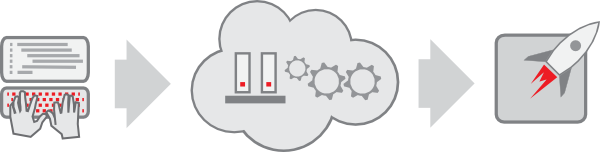
\includegraphics[scale=0.5]{./images/overview-paas.png}
    \caption{Platform as a Service overview}
\end{figure}

Red Hat is an open-source company, i.e. every project developed by Red Hat is open-source -- and so is OpenShift. OpenShift is build on RHEL\footnote{Red Hat Enterprise Linux} which is a stable Linux distribution with long-term support, it is written in Ruby programming language and it runs your application on Amazon EC2\footnote{Amazon Elastic Compute Cloud -- cloud computing platform that allows users to rent virtual computers}.

Creating your first application on OpenShift is very straightforward. First, you choose a type of application which is called a cartridge in OpenShift terminology. You can choose from a variety of cartridges including, for example, JBoss Application Server, Tomcat 7, Ruby on Rails and Django, or you can choose a Do It Yourself cartridge and set up the whole environment yourself. Once you have done that, you can choose a public URL, a source code repository, gears and scaling. A gear is container with limited resources that runs your application, i.e. virtual server. By default, you can only choose the default small gear. If you pay a monthly fee, you can choose medium or large gear with more resources at your disposal. Scaling allows your application to be load-balanced, i.e. if your applications' traffic increases, OpenShift will allocate more gears. When you have your application created, you can do some basic configuration through the web interface or you can add another cartridge to your application, e.g. a database or Cron. If you need to connect to the server where your application runs, you can open a Secure Shell session (supposing you set up your public RSA key). This overall flexibility makes it easy to deploy your application without any fuss and decreases time spent managing software and hardware, so from that point of view, it makes sense to use OpenShift even if you have no choice but to use Do It Yourself cartridge.

If setting up a new OpenShift application is simple, deploying one is even more simple. You just push the application's source code to either the repository you specified or the repository that was created for you. You might need to set some properties in your application (e.g. database credentials), though. Fortunately, OpenShift exports all needed properties as environment variables so that you could access them via the API of your programming language and use them wherever necessary. If you need to inject or modify some environment variables at some point (e.g. before or after build), you can use action hooks. These lifecycle hooks allows you to execute any kind of shell script at a certain point in time, for example, you might want to append a property to the \texttt{JAVA\_OPTS} environment variable just before the build of your application. To do that, you put following script in \texttt{\$\{project.dir\}/.openshift/action\_hooks/pre\_build}:

\begin{verbatim}
#!/bin/bash
export JAVA_OPTS="$JAVA_OPTS -DsomeProperty=true"
\end{verbatim}

The script above gets executed directly, so you can use PHP, Python, Ruby or any other interpreted programing language.

\section{Others}

There are a lot of other technologies used in the Thesis Management System, to keep it short, the author will describe them just briefly.

\begin{itemize}
    \item Spring Security -- a framework that provides authentication and authorization for Java
    \item Searchable -- Grails plugin that adds search functionality based on Compass and Apache Lucene\cite{searchable-documentation}
    \item JQuery -- the most popular JavaScript framework
    \item LESS -- CSS preprocessor
    \item Twitter Bootstrap -- CSS framework that is the most popular project on GitHub
\end{itemize}


\chapter{Project Architecture and Design}

In the following text, the author will describe the architecture and design of the Thesis Management System including functional and non-functional requirements, and the domain model. The author will also depict some design parts with UML\footnote{Unified Modeling Language} 2.0 diagrams that were modeled with Visual Paradigm tool\cite{visual-paradigm-homepage}, however, the UML diagrams are not to be regarded as blueprints of the system, but rather as sketches, and as such, some information that the author considers irrelevant or obvious are let out. This is allowed as stated by Martin Fowler in his book UML Distilled\cite{fowler-uml}.

\section{Functional Requirements}

\begin{enumerate}
    \item User management\\
    The system allows to create, read, update and delete (CRUD) users. User contains fields full name, email and password.

    \item Registration\\
    Anonymous users can sign up only with emails hosted at configured domain addresses.

    \item Log In\\
    Anonymous users can sign in using email and password.

    \item Site configuration\\
    Administrator can configure certain aspects of the system, like allowed email domain addresses, site announcement and the terms of use.

    \item Thesis topic management\\
    The system allows to CRUD thesis topics. Topic contains fields title and description in two languages.

    \item Category management\\
    The system allows to CRUD categories. Category contains fields title and description.

    \item Topic can be added to categories.\\
    One topic can be added to one or more categories, which allows users to browse topics by categories.

    \item Tags can be assigned to topics\\
    There can be zero or more tags assigned to one topic.

    \item Topic contains field for a leader\\
    The leader of a topic has the authority to manage topics created by them.

    \item University management\\
    The system allows to CRUD universities. University contains a field for the name of the university.

    \item Topic contains a field for the list of universities\\
    This field contains the list of universities that a topic is offered to. One topic can be offered to one or more universities.

    \item Topic contains a field for the list of supervisors\\
    This field contains the list of university supervisors, each supervisor is assigned a university that they supervise at. One topic can have zero or more university supervisors.

    \item Topic contains a field for the list of types\\
    This field contains the list of thesis types (i.e. diploma, bachelor). Topic can have one or more types.

    \item Application management\\
    The system allows to CRUD applications.

    \item Students can apply for topics\\
    The applicant chooses the thesis type and the university that they apply to.

    \item Applications can be approved\\
    To approve an application, the leader or a supervisor must create a new thesis.

    \item Topic can be enabled or disabled\\
    When a topic is disabled, students cannot apply for it.

    \item Topics can be filtered\\
    The system allows to filter topics by university, type, leader or title.

    \item Thesis management\\
    The system allows to CRUD theses. Thesis contains fields title, description, thesis topic, assignee, supervisor, abstract, type and university.

    \item Tags can be assigned to theses\\
    There can be zero or more tags assigned to one thesis.

    \item Thesis contains a field for status\\
    Status can be either `in progress', `finished', `failed' or `postponed'.

    \item Thesis contains a field for grade\\
    One of A, B, C, D, E or F.

    \item Supervisors can select universities they supervise at for each topic

    \item Supervisors can add private notes to theses

    \item Authenticated user can subscribe for topics and theses\\
    The system sends notifications to all subscribers of a topic or a thesis when a change is made to it.

    \item Authenticated user can unsubscribe from topics and theses

    \item Theses can be filtered\\
    The system allows to filter theses by title, supervisor, assignee, status, grade, type or university.

    \item Theses and topics can be filtered by tags\\
    The system allows to list theses or topics that contain a particular tag.

    \item File management for theses\\
    The system allows to upload files to theses.

    \item Discussion for topics and theses\\
    Logged in users can comment on topics and theses.

    \item Private comments\\
    Users with certain authority can create comments that are not visible to students and guests.

    \item Full text search\\
    Theses and topics can be searched by a full text search engine.

    \item Frequently Asked Questions (FAQ) management\\
    The system allows to CRUD Frequently Asked Questions. One frequently asked question contains fields question, answer and locale.

\end{enumerate}

\subsection{Use Case Diagram}

\begin{figure}[H]
    \centering
        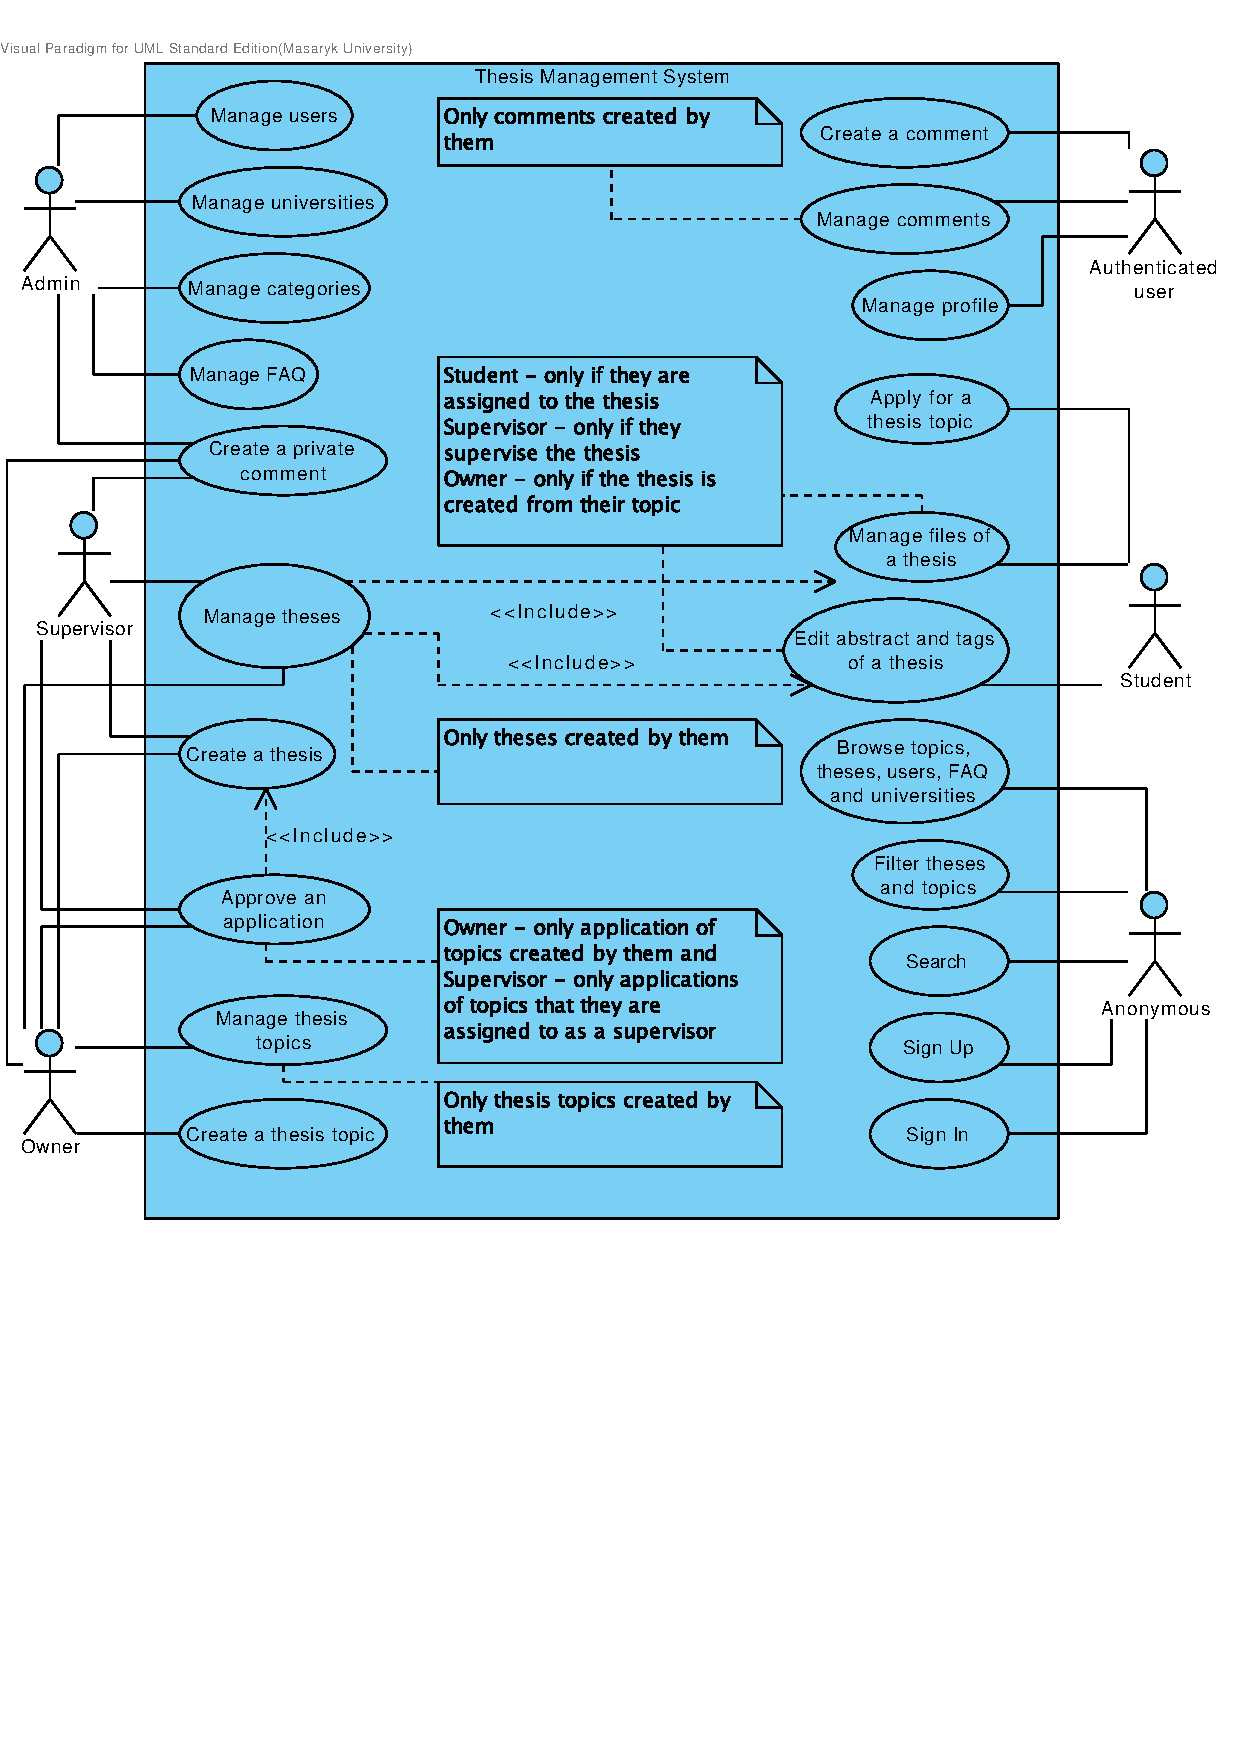
\includegraphics[trim=0 190 10 30, clip, keepaspectratio, width=\textwidth]{./images/use-case.pdf}
    \caption{Use case diagram of the Thesis Management System}
    \label{fig:use-case}
\end{figure}

\section{Non-Functional Requirements}

\begin{enumerate}
    \item Grails platform\\
    The system is implemented using platform Grails.

    \item Authentication and authorization\\
    The system is secured and there are four roles -- \textbf{Administrator} that can manage users, categories, FAQ and universities, \textbf{Leader} that can create topics and manage topics created by them, \textbf{Supervisor} that can create theses and manage theses created by them and \textbf{Student} that can apply for topics.

    \item Performance\\
    The system offers reasonable performance at least up to five hundred created topics, theses, users and universities.

    \item Deployment\\
    The system is deployed on OpenShift using any cartridge other than Do It Yourself.

    \item License\\
    The system is licensed under a GPL compatible license.

    \item Backup\\
    There is available a shell script for backing up the database.

    \item Internationalization and localization\\
    The system is internationalized and localized in English and Czech.

    \item Software development methodology\\
    The system is developed iteratively and incrementally.

\end{enumerate}

\section{Domain Model}

Designing the domain model is the most important step when developing an information system. It is also the most difficult one, because you usually cannot easily make changes in the domain model after you implemented the application logic around it. You can, however, add some domain model elements that the already-designed elements do not relate to. For example, if you design an entity \texttt{User}, you can implement it and easily add new entity \texttt{Group} later on if the \texttt{Group} is the owner of the relationship, see fig. \ref{fig:user-group-owner-example}. If the \texttt{User} is the owner of the relationship (see fig. \ref{fig:user-owner-group-example}), more refactoring is required to implement such changes (especially in case of object composition), because the fundamental API of the implemented part of the system changed.

\begin{figure}[h]
    \centering
        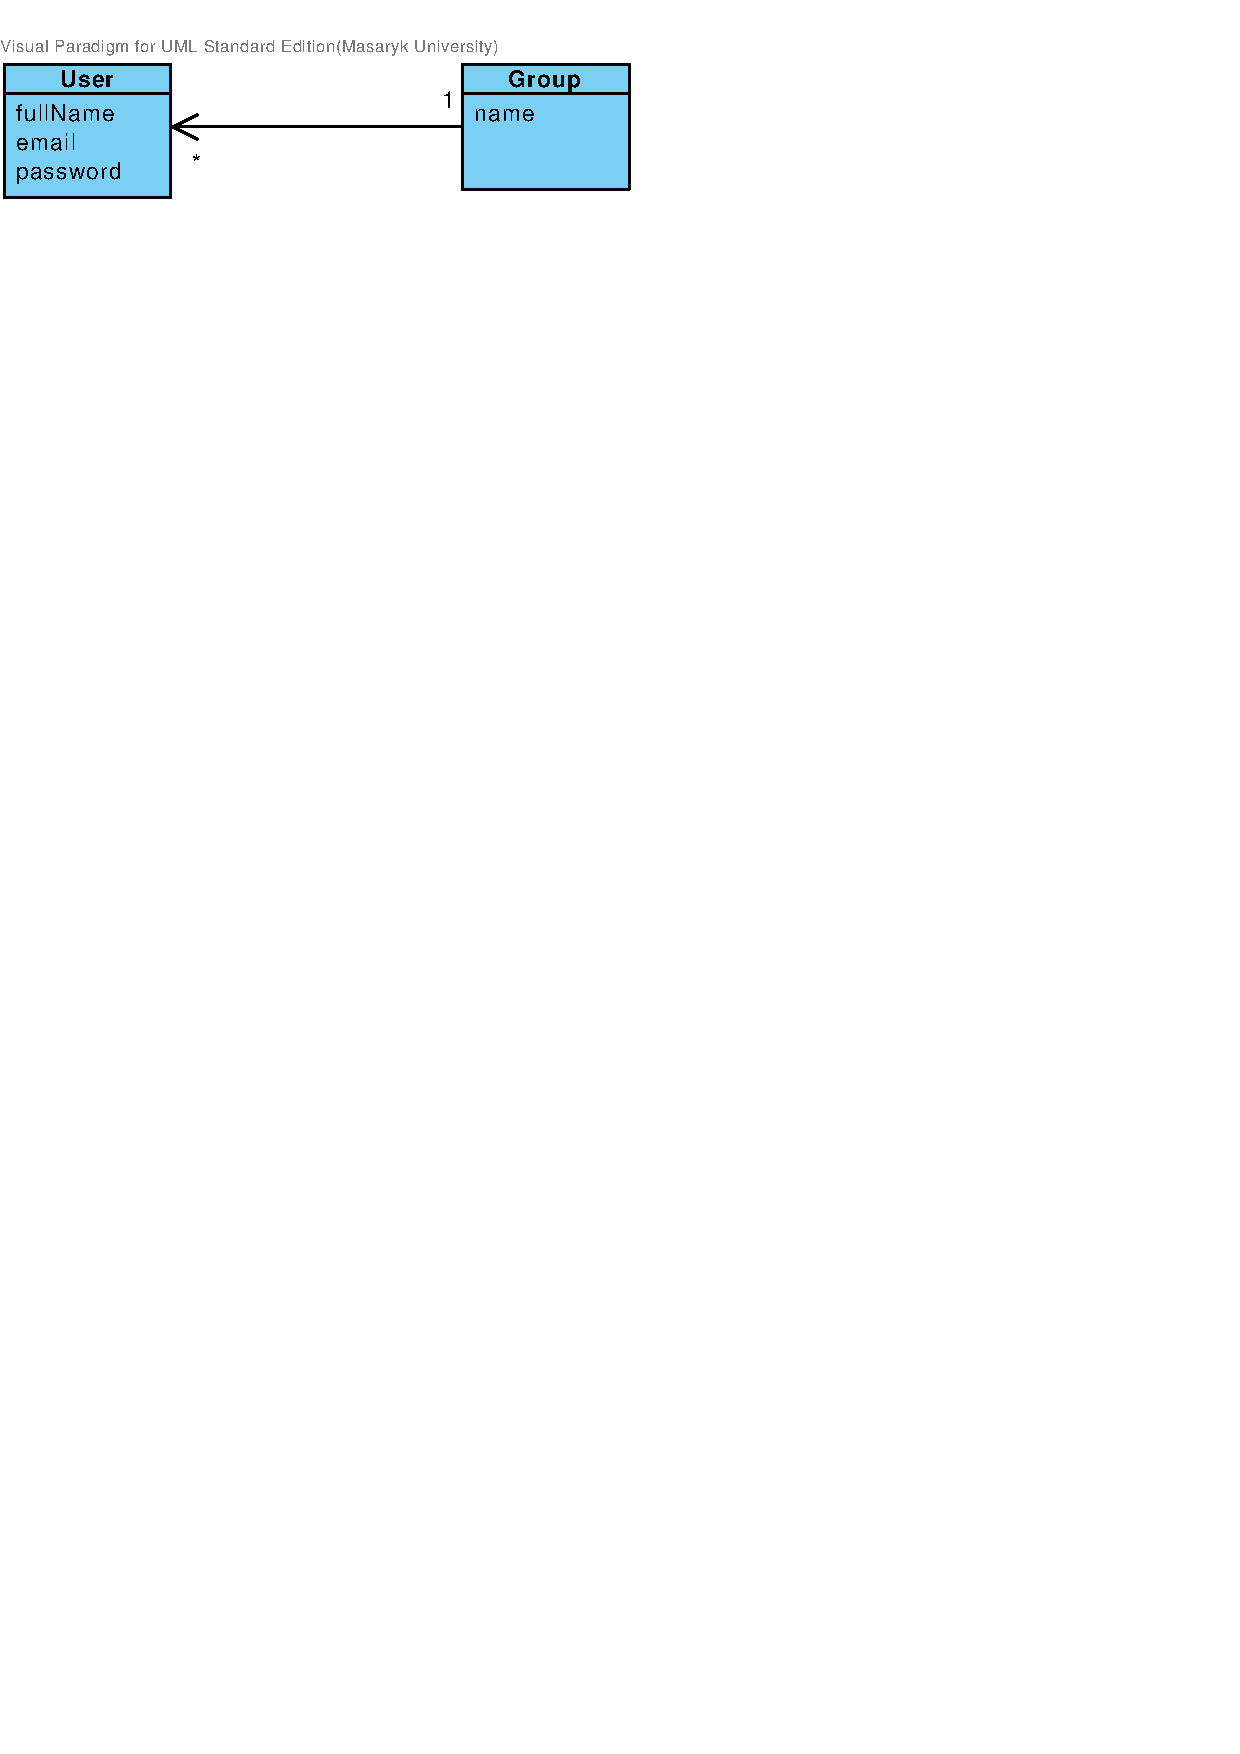
\includegraphics[trim=0 740 290 30, clip, keepaspectratio]{./images/user-group-owner-example.pdf}
    \caption{Example of domain model where \texttt{Group} owns the relationship}
    \label{fig:user-group-owner-example}
\end{figure}

\begin{figure}[h]
    \centering
        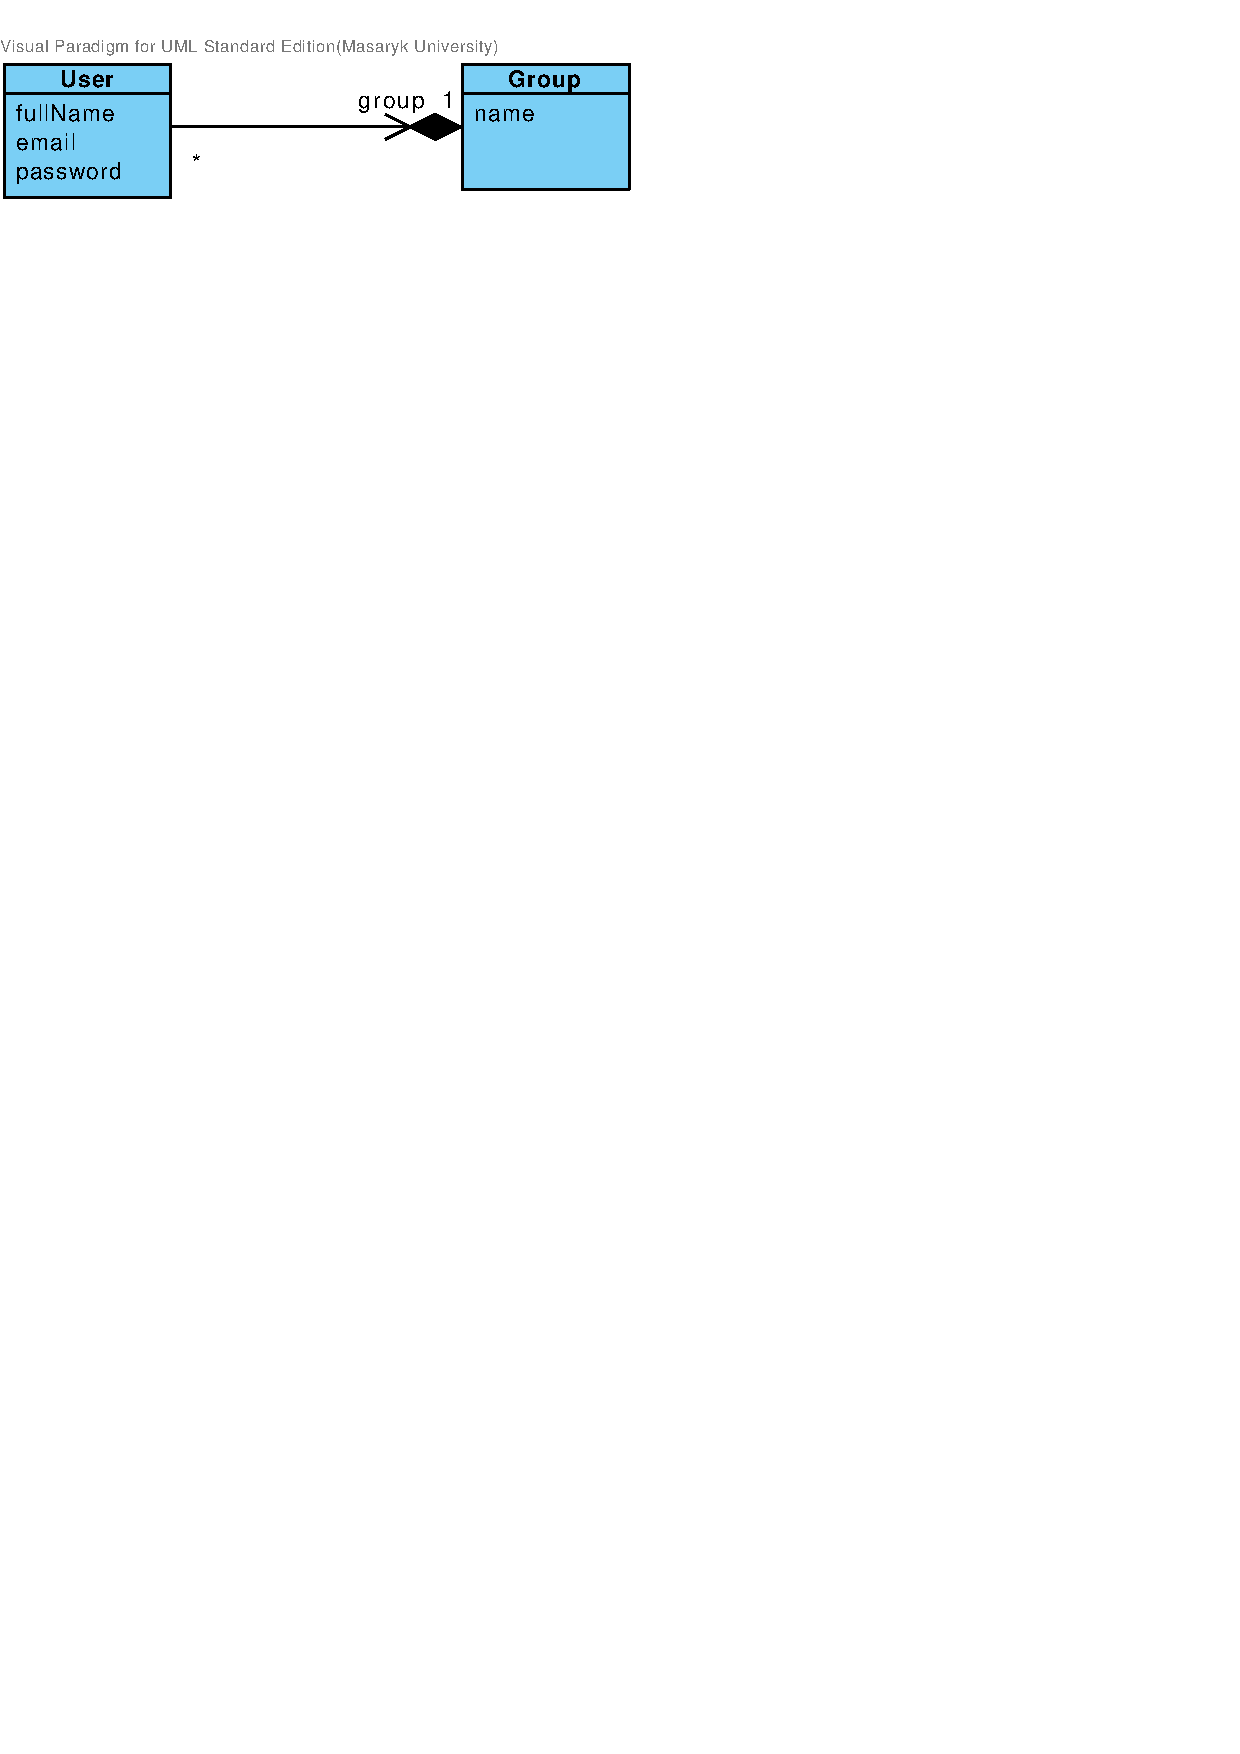
\includegraphics[trim=0 740 290 30, clip, keepaspectratio]{./images/user-owner-group-example.pdf}
    \caption{Example of domain model where \texttt{User} owns the relationship and composition is introduced}
    \label{fig:user-owner-group-example}
\end{figure}

Even more difficult can be deleting or editing attributes of an implemented entity. As a lot of refactoring is necessary to cope with such changes, a lot of new bugs is usually introduced, so it is best to avoid such changes by designing the domain model thoroughly.

Note that it is necessary to change the domain model if you implement your application incrementally. You should, however, try to minimize the changes that require the API of the implemented domain model to be changed.

\subsection{Domain Model of the Thesis Management System}

As the domain model of the Thesis Management System is very complex, the author will describe it part by part. The complete domain model can be found in the appendix A.

\subsubsection{\textbf{\texttt{User} entity}}

To fulfill the first three functional requirements, we need to register users. For that reason, we introduce entity \texttt{User} with fields \texttt{email} and \texttt{password} that serve as log in credentials and field \texttt{fullName}. We also need fields \texttt{accountLocked} to allow the administrator to lock a user account and \texttt{enabled} for registration confirmation purposes. Field \texttt{sendMail} represents the user setting that allows them to disable receiving notifications by email, and field \texttt{dateCreated} represents the date of user's registration. To implement authorization, the \texttt{User} entity needs field \texttt{roles}, which contains the list of user's authorities. Figure \ref{fig:domain-user-entity} illustrates the described model.

\begin{figure}[h]
    \centering
        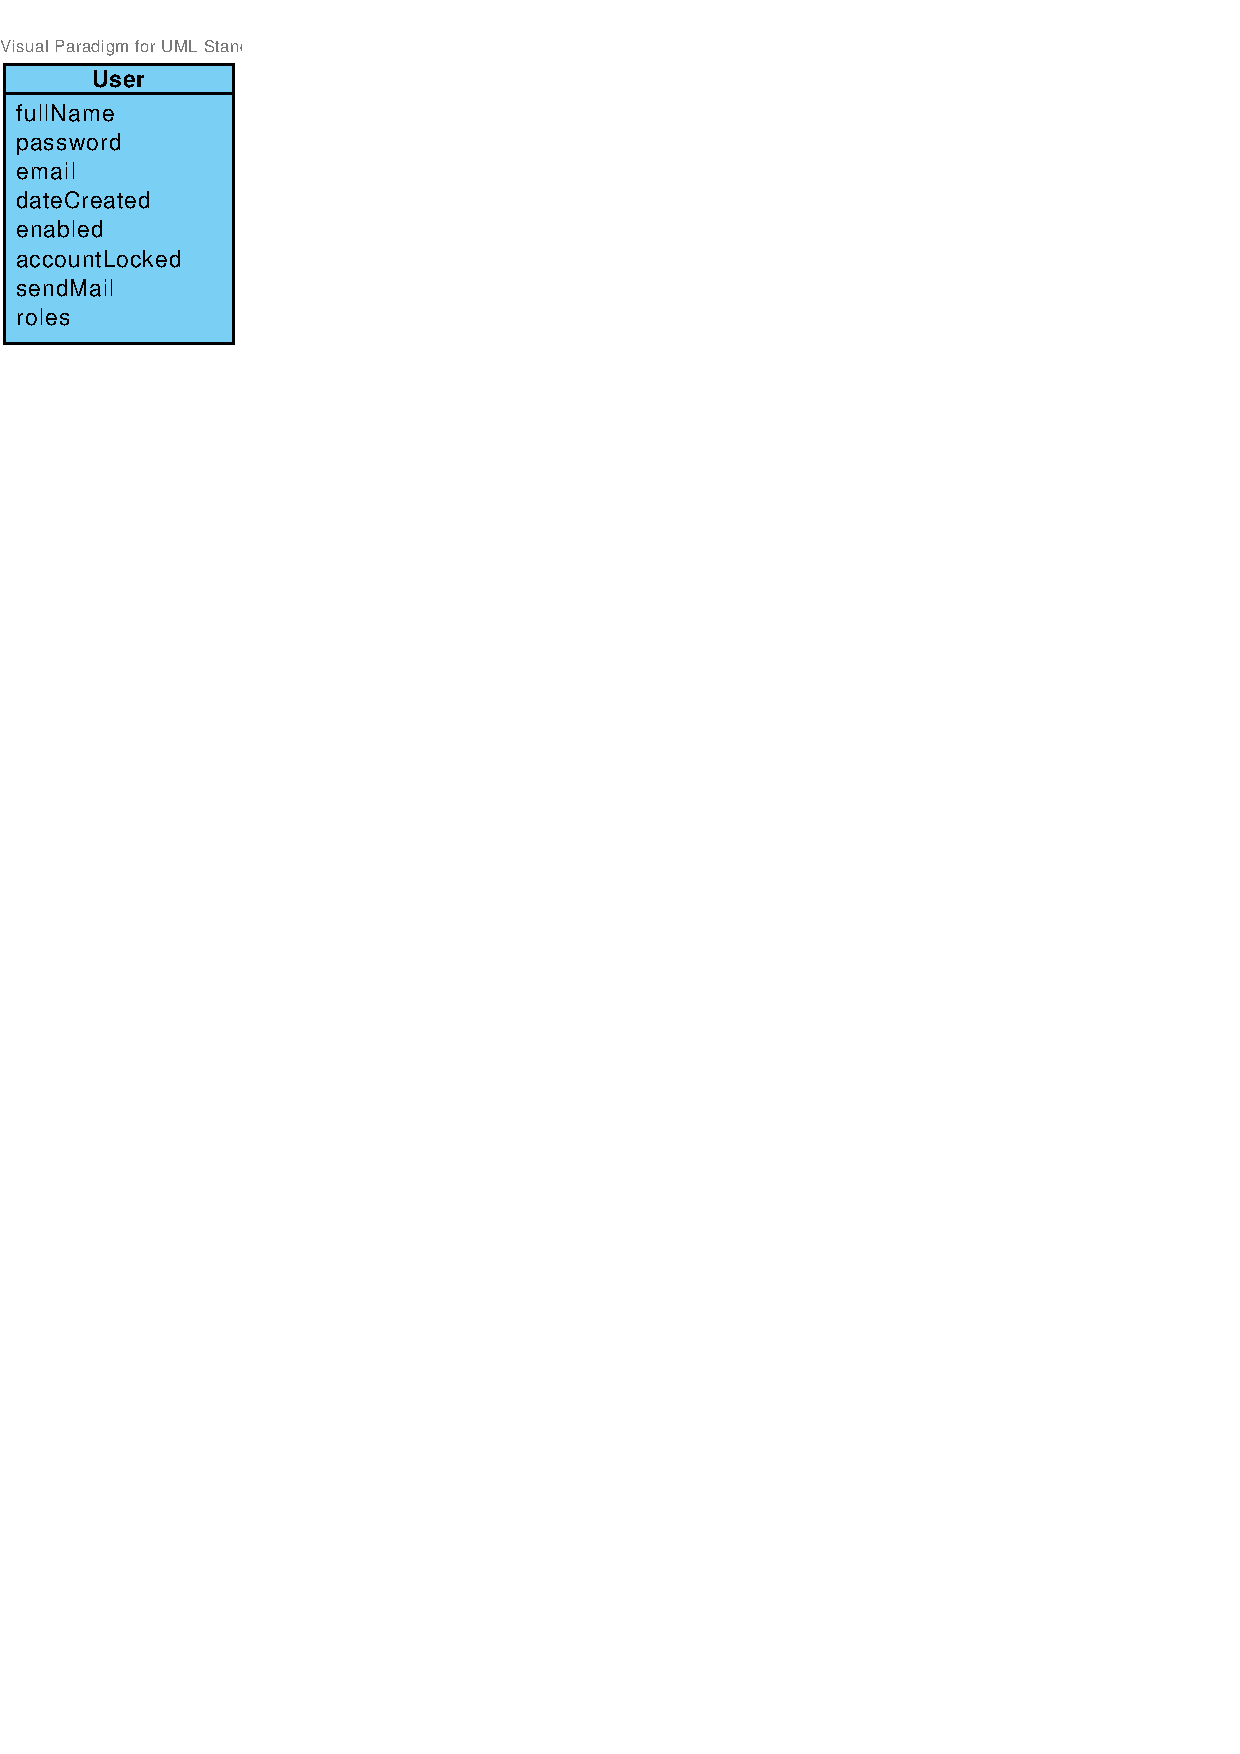
\includegraphics[trim=0 675 480 30, clip, keepaspectratio, scale=0.8]{./images/domain-user-entity.pdf}
    \caption{Model of \texttt{User} entity}
    \label{fig:domain-user-entity}
\end{figure}

\subsubsection{\textbf{\texttt{University} entity}}

To be able to keep a record of the universities that a topic is offered to, we need the entity \texttt{University} with only one field -- \texttt{name}, see Figure \ref{fig:domain-university-entity}.

\begin{figure}[h]
    \centering
        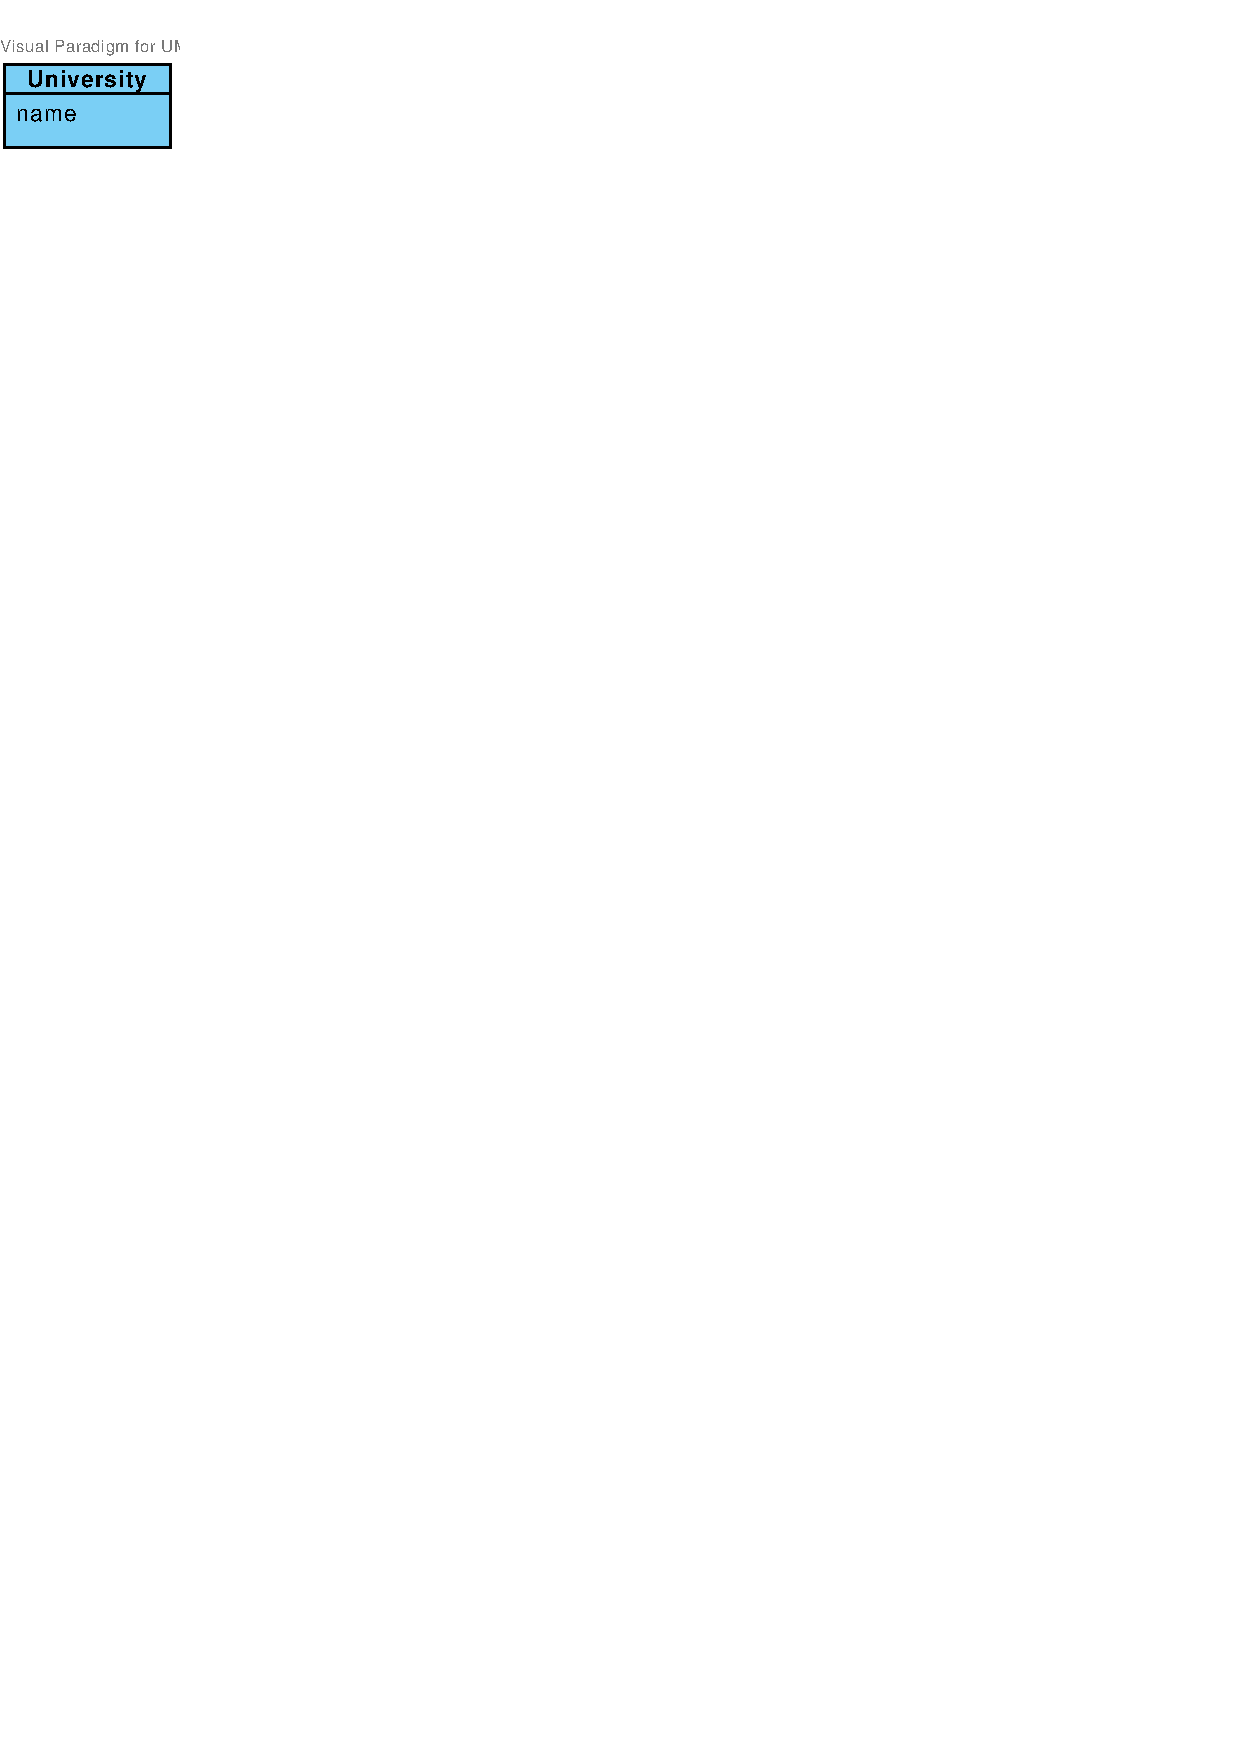
\includegraphics[trim=0 770 510 30, clip, keepaspectratio]{./images/domain-university-entity.pdf}
    \caption{Model of \texttt{University} entity}
    \label{fig:domain-university-entity}
\end{figure}

\subsubsection{\textbf{\texttt{Article}, \texttt{Comment} and \texttt{Subscription} entities}}

To allow users to add comments to topics and theses, we need an entity that represents comments. The name of the entity is, for obvious reasons, \texttt{Comment} and fields that the entity requires are:

\begin{itemize}
    \item \texttt{content} -- Represents the content of a comment.
    \item \texttt{privateComment} -- Marks private comments.
    \item \texttt{dateCreated} -- The date of creation, this field is used for sorting comments so that we could show the user comments in either descending or ascending order.
\end{itemize}

There are two association we need to create for \texttt{Comment}. First is a many-to-one association between \texttt{Comment} and \texttt{User} to be able to display the author of a comment. Second is a bit more complicated, because there are two approaches to associate comments with topics and theses. We could either create a many-to-one association between entities \texttt{Comment} and \texttt{Topic} and between entities \texttt{Comment} and \texttt{Thesis}, or we could use generalization and move the many-to-one association up from \texttt{Thesis} and \texttt{Topic} to their parent. We choose the later approach because it allows us to create another ``commentable'' entity in the future simply by making it another child of the parent entity.

The \texttt{Article} entity represents the parent entity described above. We place the field \texttt{title} on it for reasons described in the following paragraph.

The \texttt{Subscription} is only an association entity with no attributes on it, but for the sake of future improvements, we model it separately. We could, for example, allow users to choose if they want to receive email notification for a particular subscription, or let them set up what changes made to an \texttt{Article} they want to be notified about. As far as associating the entity with other entities is concerned, it is very similar to the \texttt{Comment} entity, because we need to implement subscription functionality for both topics and theses. We add the field \texttt{title} on the \texttt{Article} entity because we want to show subscribers the name of the \texttt{Article} that changed.

Described model is illustrated in Figure \ref{fig:domain-article-comment-subscription-entities}.

\begin{figure}[h]
    \centering
        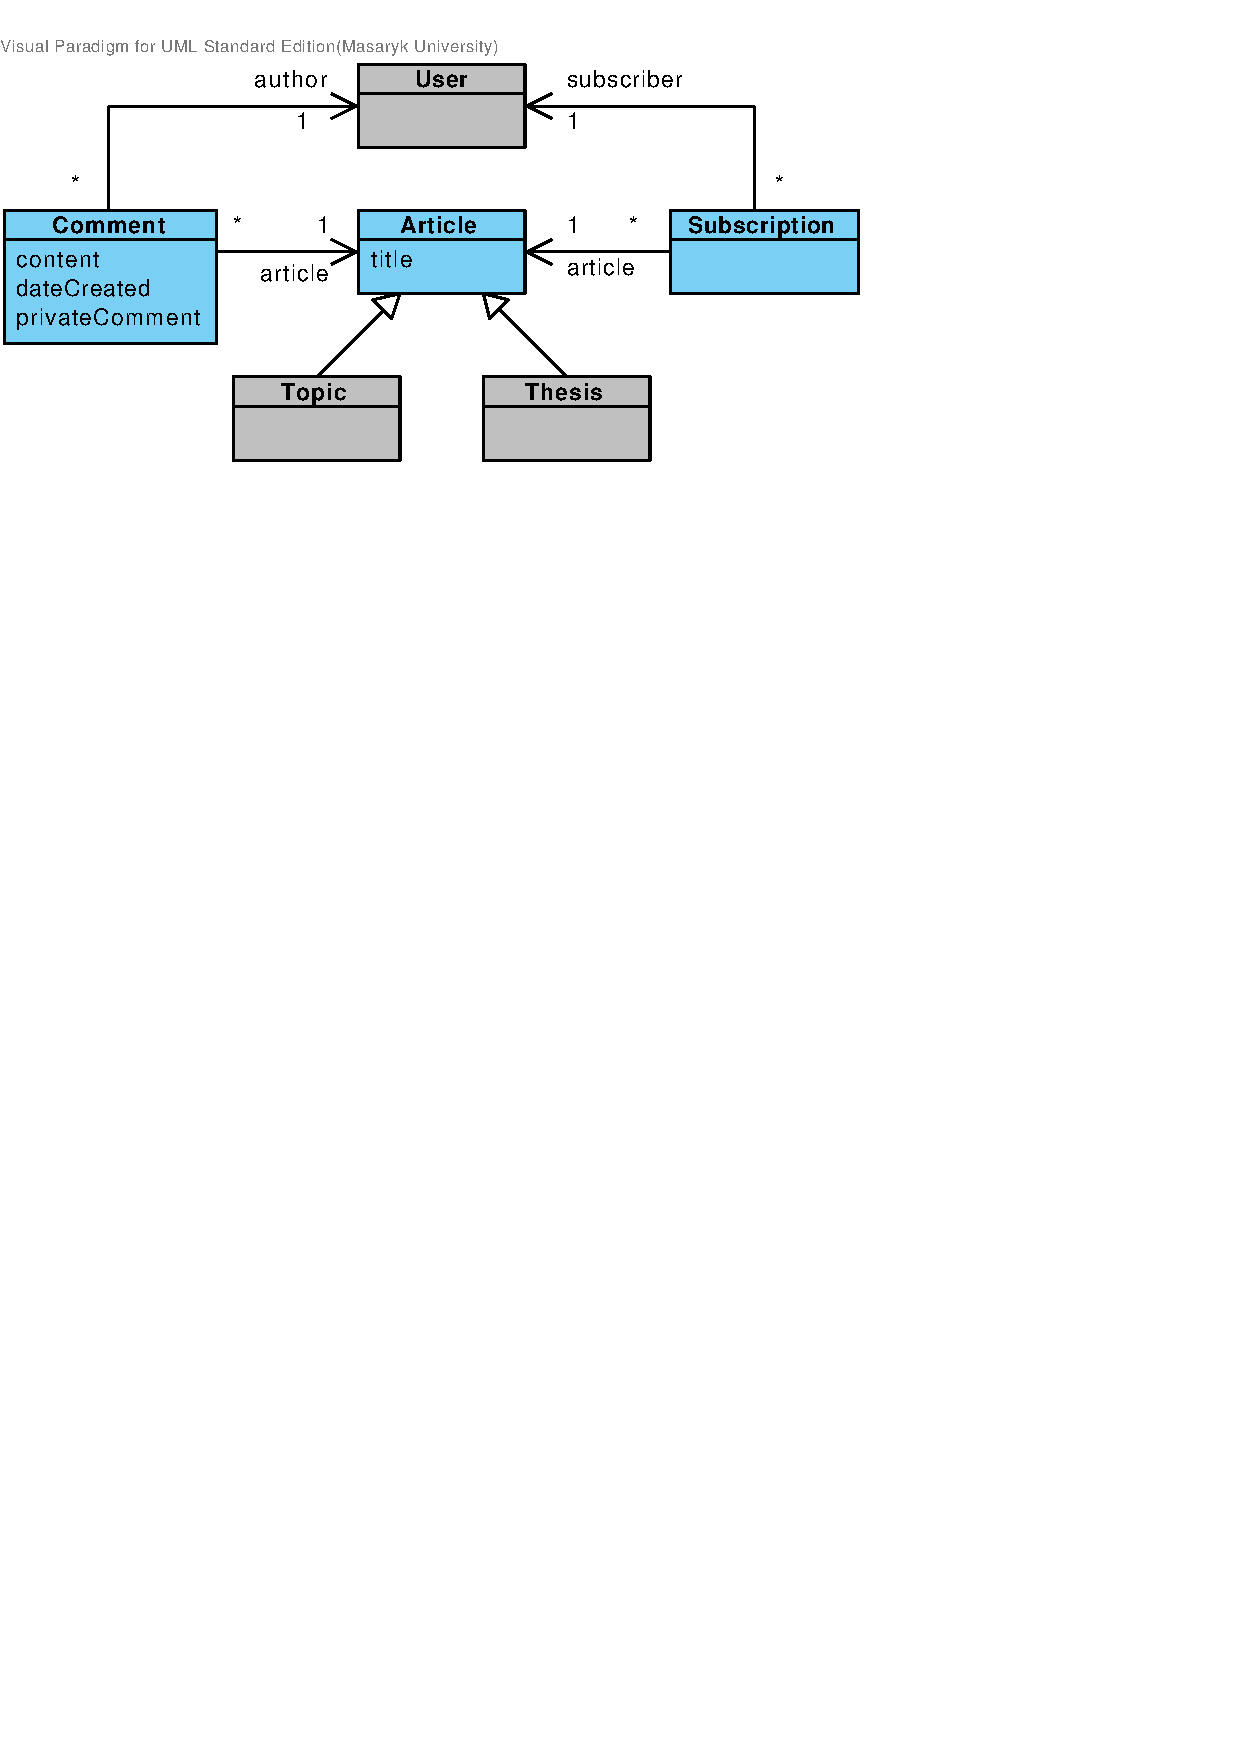
\includegraphics[trim=0 620 180 30, clip, keepaspectratio, width=\textwidth]{./images/domain-article-comment-subscription-entities.pdf}
    \caption{Model of \texttt{Article}, \texttt{Comment} and \texttt{Subscription} entities}
    \label{fig:domain-article-comment-subscription-entities}
\end{figure}

\subsubsection{\textbf{\texttt{Feed} and \texttt{Notification} entities}}

Entities \texttt{Feed} and \texttt{Notification} are quite closely related to the \texttt{Subscription} entity even though they are not directly associated. When a change is made to a topic or a thesis, the subscribers are notified by email and by a notification within the system. Emails are stored by the email hostings, but the notifications need to be stored in the database of the Thesis Management System, because they must be available to users when they visit the system.

Now, there are several ways to implement such functionality, but the most notable ones are the following two. The first approach is to create a \texttt{Notification} entity with the \texttt{message} field that represents the content of the notification, and associate it with the \texttt{User} entity that represents the subscriber. This approach is favorable because it is simple, however, it creates unnecessary redundancy in the database as a new notification with the same \texttt{message} is created for every subscriber. The second approach, which is used in the Thesis Management System, is to create another entity \texttt{Feed} and move the \texttt{message} field into it. The later approach is also more suitable if we want to show the user a notification according to their locale setting. 

Figure \ref{fig:domain-feed-notification-entities} illustrates the model of this part of the system. Since we want the notifications to be localized, the \texttt{Feed} entity has fields \texttt{messageCode}, which represents the code of the massage to be displayed as a notification, \texttt{args}, which represents the arguments of the message, and \texttt{dateCreated}, which allows us to sort the notifications to show users the latest notifications first. The \texttt{Feed} entity is also associated with the \texttt{User} entity, which represents the user who triggered the creation of the feed. This allows us to find user's activity.

The \texttt{Notification} entity is basically an association entity between entities \texttt{User} and \texttt{Feed}. The field \texttt{seen} represents status of a notification, i.e. if the user has already seen the notification or not.

\begin{figure}[h]
    \centering
        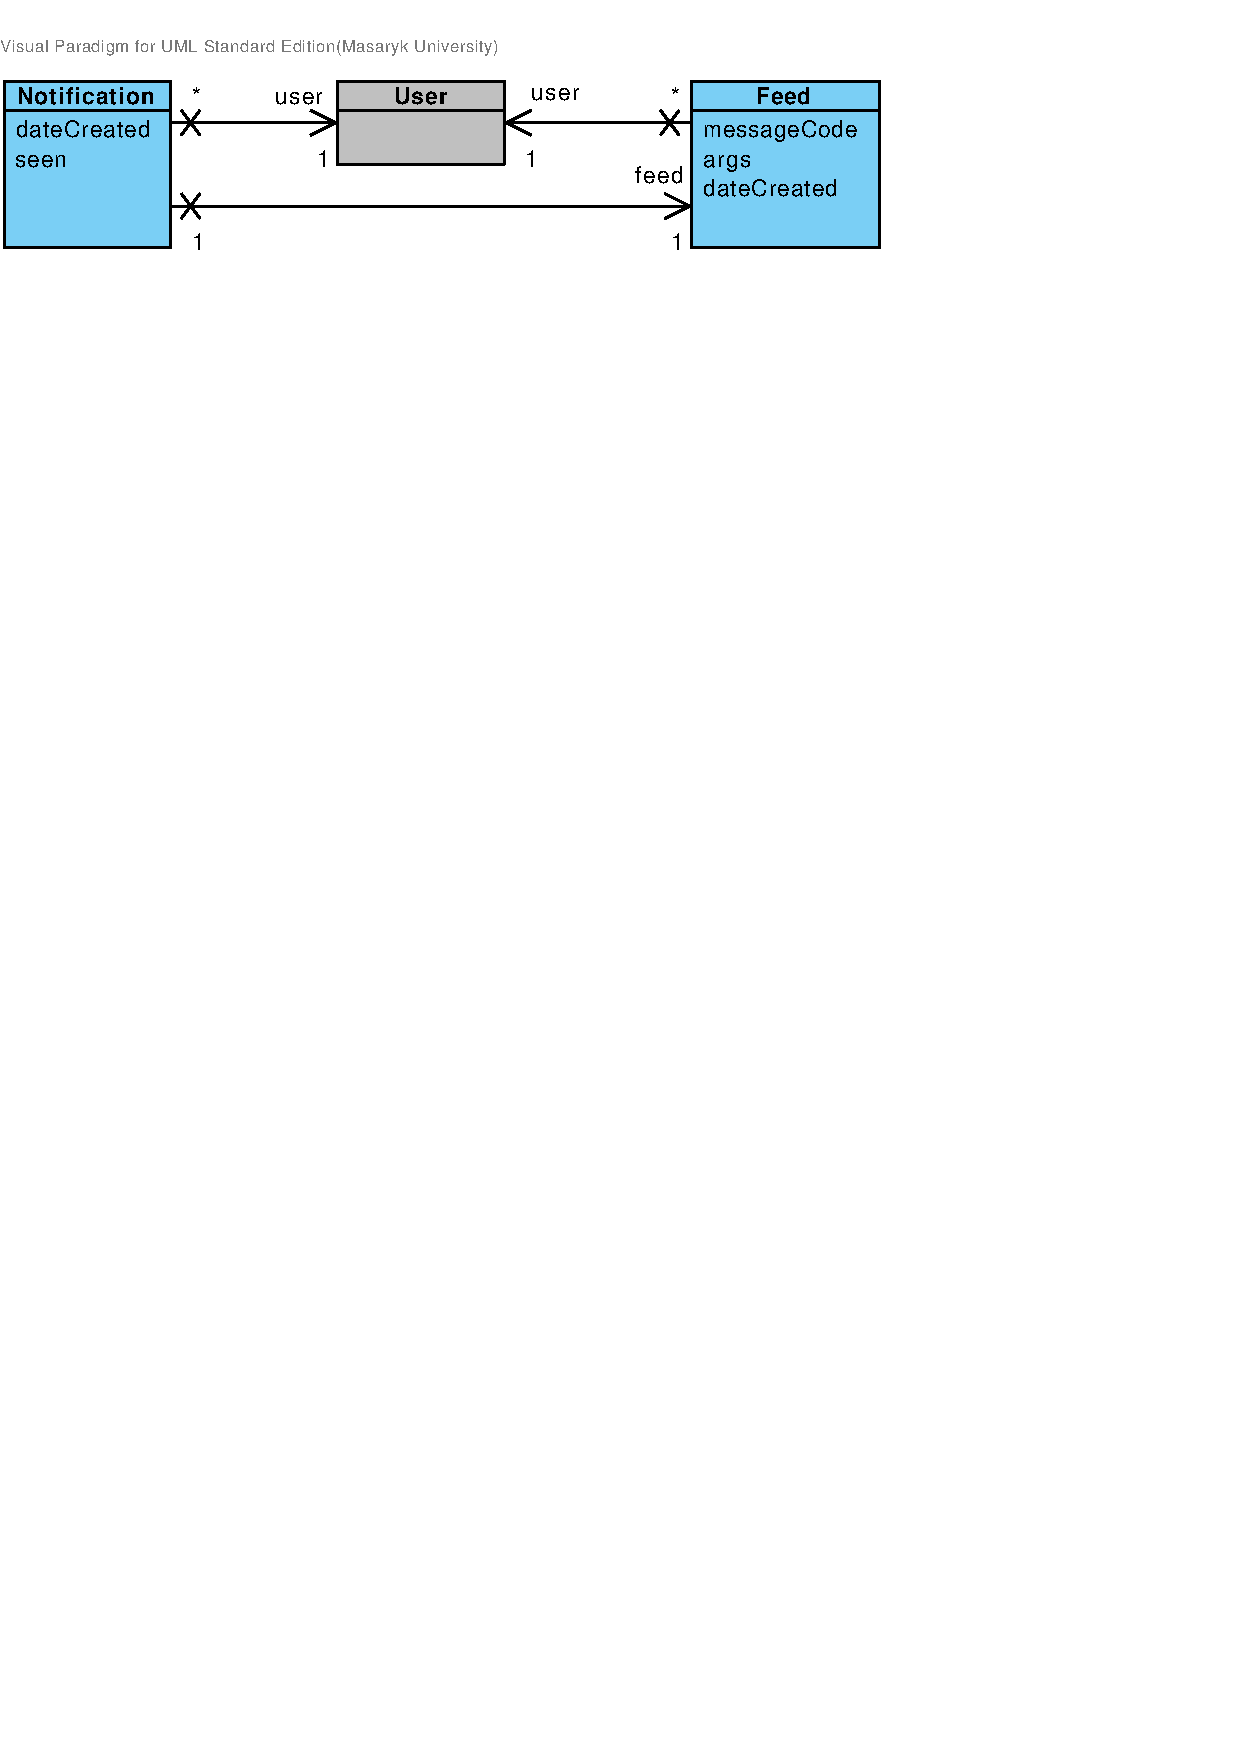
\includegraphics[trim=0 720 170 30, clip, keepaspectratio, width=\textwidth]{./images/domain-feed-notification-entities.pdf}
    \caption{Model of \texttt{Feed} and \texttt{Notification} entities}
    \label{fig:domain-feed-notification-entities}
\end{figure}

\subsubsection{\textbf{\texttt{Tag} entity}}

The most common way of implementing tags in an information system is to place collection of simple strings in an entity. We chose a different approach for the Thesis Management System, though. We introduced a separate entity \texttt{Tag} that contains a simple field \texttt{title}. Making the \texttt{Tag} entity separate makes it easy to add new fields on it in the future, e.g. \texttt{description}, and it is easier to aggregate, for example, the number of all tags used in the system. Figure \ref{fig:domain-tag-entity} depicts the model.

\begin{figure}[h]
    \centering
        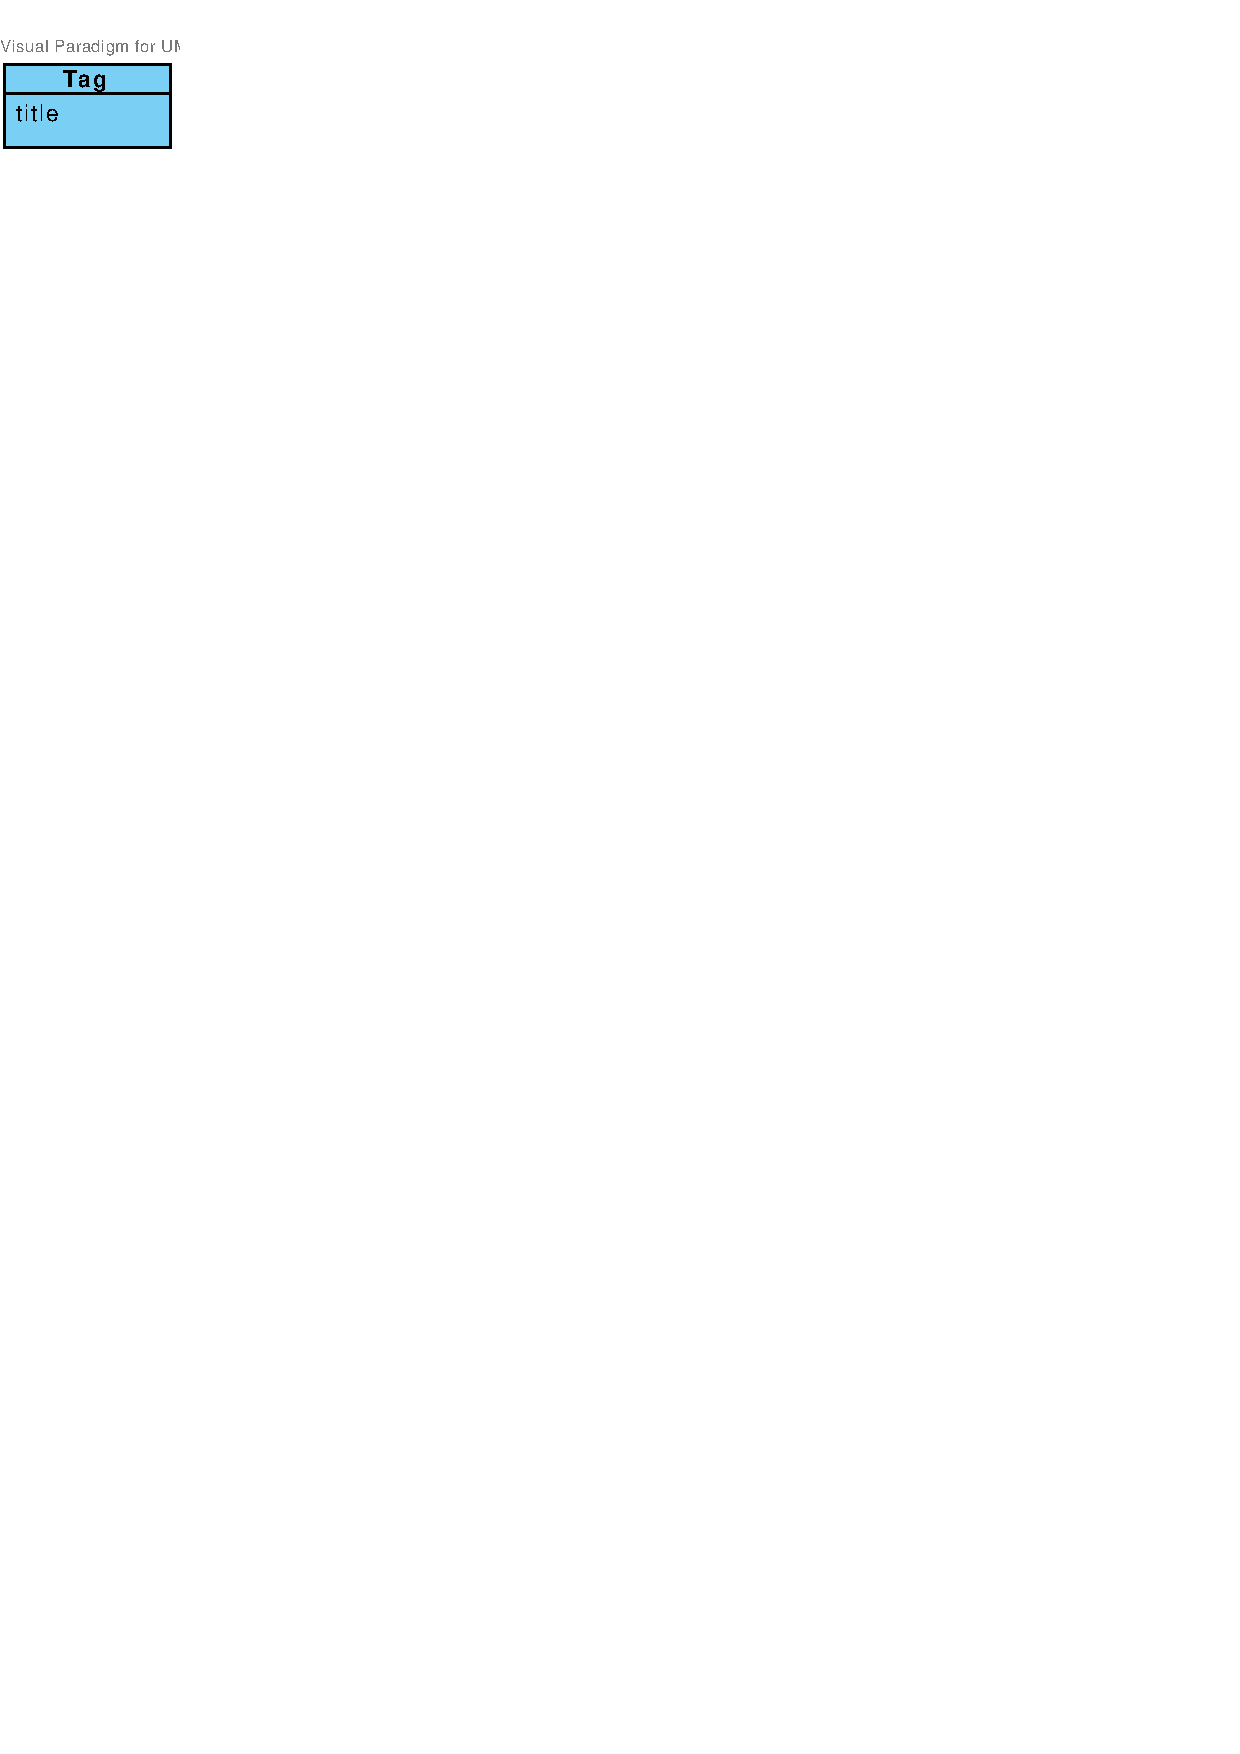
\includegraphics[trim=0 770 510 30, clip, keepaspectratio]{./images/domain-tag-entity.pdf}
    \caption{Model of \texttt{Tag} entity}
    \label{fig:domain-tag-entity}
\end{figure}

\subsubsection{\textbf{\texttt{Topic}, \texttt{Category} and \texttt{Supervision} entities}}

\texttt{Topic} is the most important entity in the system because it represents the topic of a thesis. It is a child entity of the \texttt{Article} entity, which means that the \texttt{title} field is included in the \texttt{Topic} entity automatically. Description of the other fields follows:

\begin{itemize}
    \item \texttt{secondaryTitle} -- Represents the title of the topic in a different language (e.g. Czech, Slovak).
    \item \texttt{lead} -- Lead paragraph, is displayed on the page with the list of topics.
    \item \texttt{Description} -- Description of the topic.
    \item \texttt{secondaryDescription} -- Represents the description of the topic in a different language.
    \item \texttt{dateCreated} -- The date of creation of the topic.
    \item \texttt{enabled} -- Flag which marks a topic that is enabled or disabled, i.e. students can(not) apply for it.
    \item \texttt{types} -- Collection of types of the topic (e.g. bachelor, diploma).
\end{itemize}

The \texttt{Topic} entity also has a many-to-many association with the \texttt{Tag} entity and the \texttt{User} entity, which represents the leader of the topic, i.e. the user who created the topic and is in charge of it. The association with the \texttt{University} entity is necessary to keep a record of universities that the topic is offered to, i.e. students of which universities can apply for it.

Another requirement of the system is to place topics in categories. Categories are represented by the \texttt{Category} entity, which has only two fields -- the \texttt{name} field, which represents the name of the category and the \texttt{description} field, which is self-explanatory. The \texttt{Topic} entity is associated with the \texttt{Category} entity in a many-to-many manner. In the first stages of the design, we expected the categories to be hierarchical, i.e. a category could have several subcategories, but we decided to abolish such approach as it would place unnecessary overhead on the database.

The most difficult part of the system was to design the requirement allowing topics to list university supervisors. There are zero or more supervisors in one topic, but one supervisor can supervise a topic at multiple universities, which means that the supervisors cannot be associated with the \texttt{Topic} entity directly. Instead, we introduced the \texttt{Supervision} entity, which is basically an association entity without any fields representing a supervisor associated with a university.

Described design is depicted in Figure \ref{fig:domain-topic-category-supervision-entities}.

\begin{figure}[h]
    \centering
        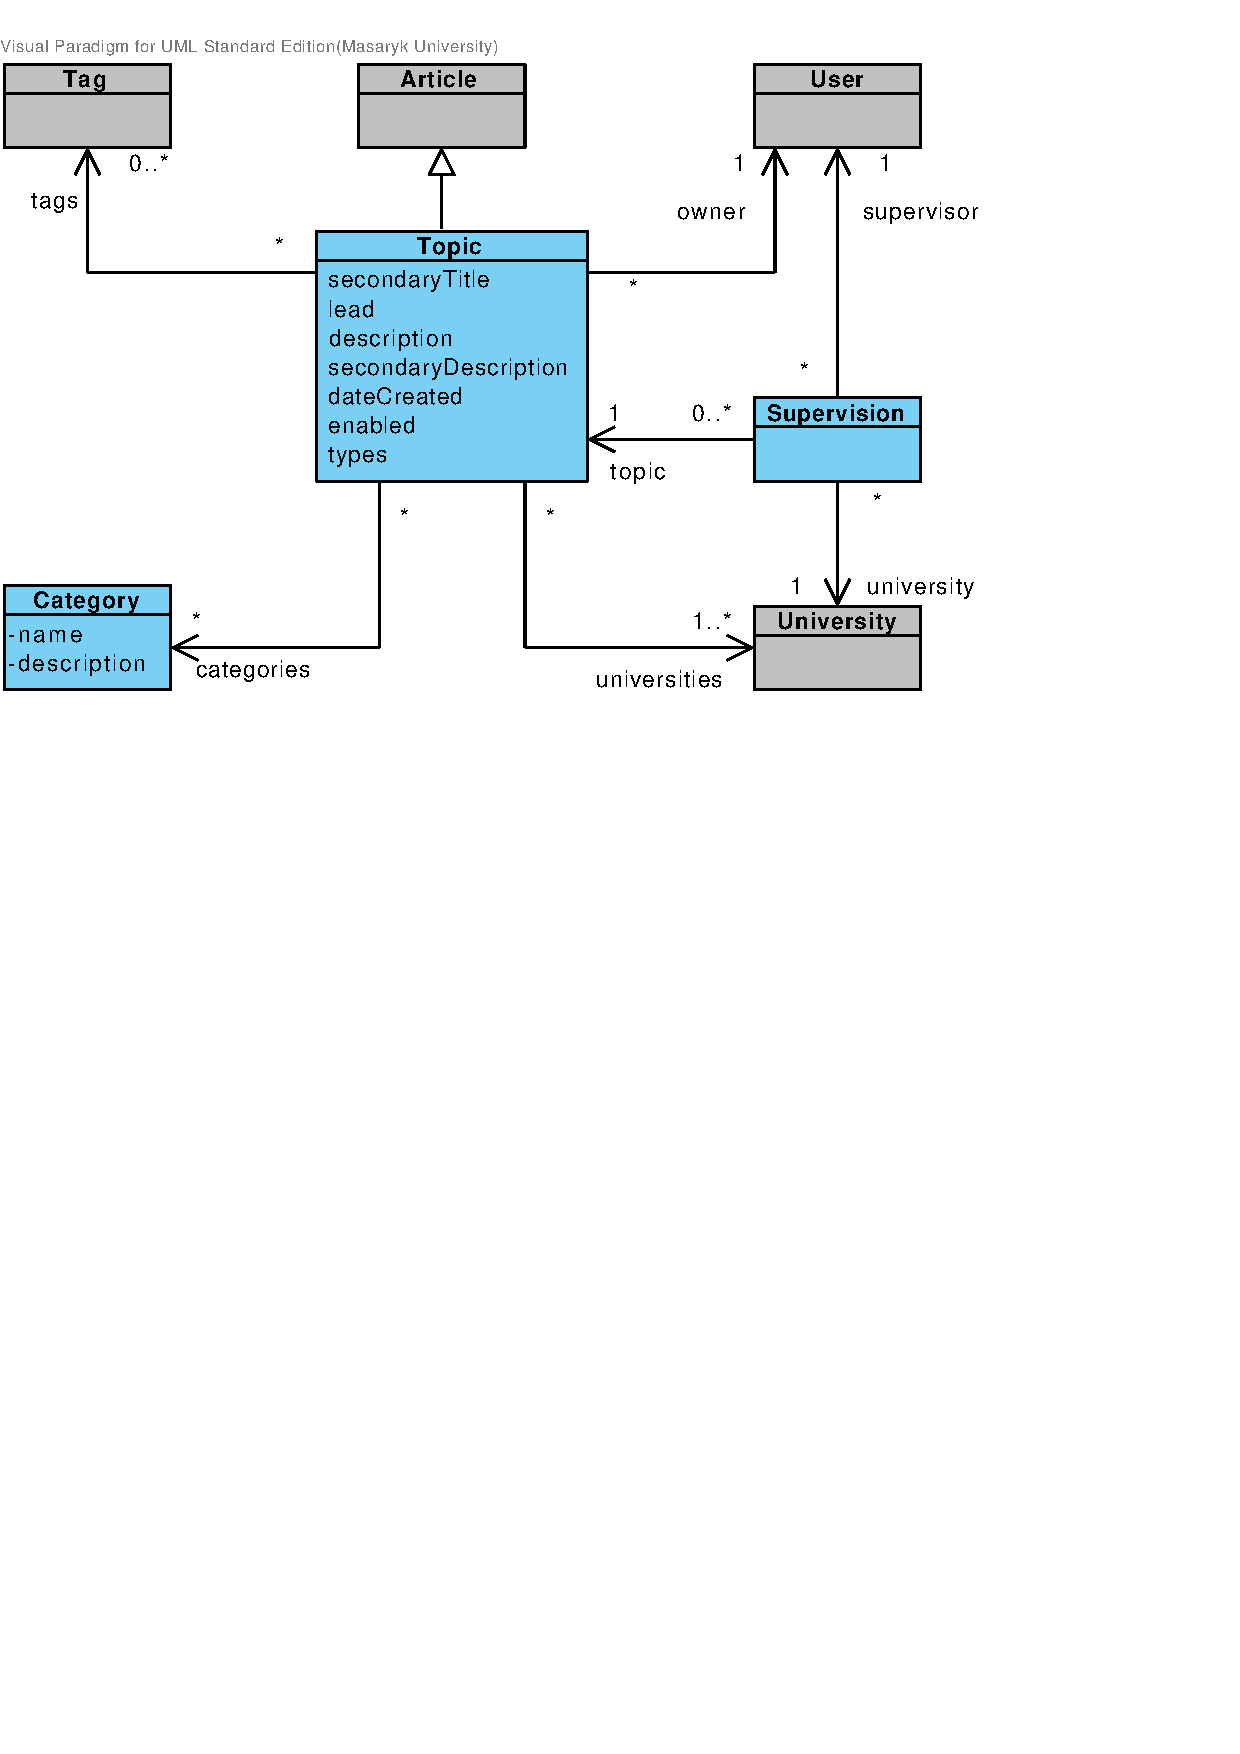
\includegraphics[trim=0 510 120 30, clip, keepaspectratio, width=\textwidth]{./images/domain-topic-category-supervision-entities.pdf}
    \caption{Model of \texttt{Topic}, \texttt{Category} and \texttt{Supervision} entities}
    \label{fig:domain-topic-category-supervision-entities}
\end{figure}

\subsubsection{\textbf{\texttt{Thesis} entity}}

The second most important entity of the system is the \texttt{Thesis} entity, it represents an academic project of a student and it is associated with the \texttt{Topic} entity. There can be multiple theses created from one topic for several reasons:

\begin{itemize}
    \item One topic can be intended for several students (for example when the topic is too difficult for one student), which means that a thesis for each student needs to be created.
    \item The topic is offered in more than one semester.
    \item The student that was assigned to the thesis of a topic failed to finish with a satisfactory result and the topic has to be offered again.
\end{itemize}

This means that the cardinality of the association with the \texttt{Topic} entity must be a many-to-one one.

The \texttt{Thesis} entity is, as well as the \texttt{Topic} entity, a child of the \texttt{Article} entity, which takes care of the title, comments and subscriptions. Theses are not required to be stored in two languages, which means that there is no need for both the secondary title and the secondary description. There are several other fields required, though:

\begin{itemize}
    \item \texttt{description} -- Represents the \emph{official} description of a thesis.
    \item \texttt{status} -- Status of a thesis, which can be either `in progress', `finished', `failed' or `postponed'.
    \item \texttt{grade} -- If the thesis is finished, a grade must be awarded. The grade can be one of the following: A, B, C, D, E, F.
    \item \texttt{abstract} -- The abstract of a thesis provided by the assigned student.
    \item \texttt{dateCreated} -- The date of creation of a thesis.
    \item \texttt{type} -- The type of a thesis, which can be for example `bachelor' or `diploma'.
    \item \texttt{notes} -- A field for the supervisor where they can leave notes related to the thesis.
\end{itemize}

The student that is assigned to a thesis and the supervisor are represented by the associations with the \texttt{User} entity and the thesis university is represented by the one with the \texttt{University}. The tags of a thesis are designed the same way as with the \texttt{Topic} entity. The reason why the association with the \texttt{Tag} entity is not moved up to the \texttt{Article} entity is because in the future, there might be added a functionality for management of school projects that does not require tags, but requires the functionality provided by the \texttt{Article} entity.

Figure \ref{fig:domain-thesis-entity} illustrates this model.

\begin{figure}[h]
    \centering
        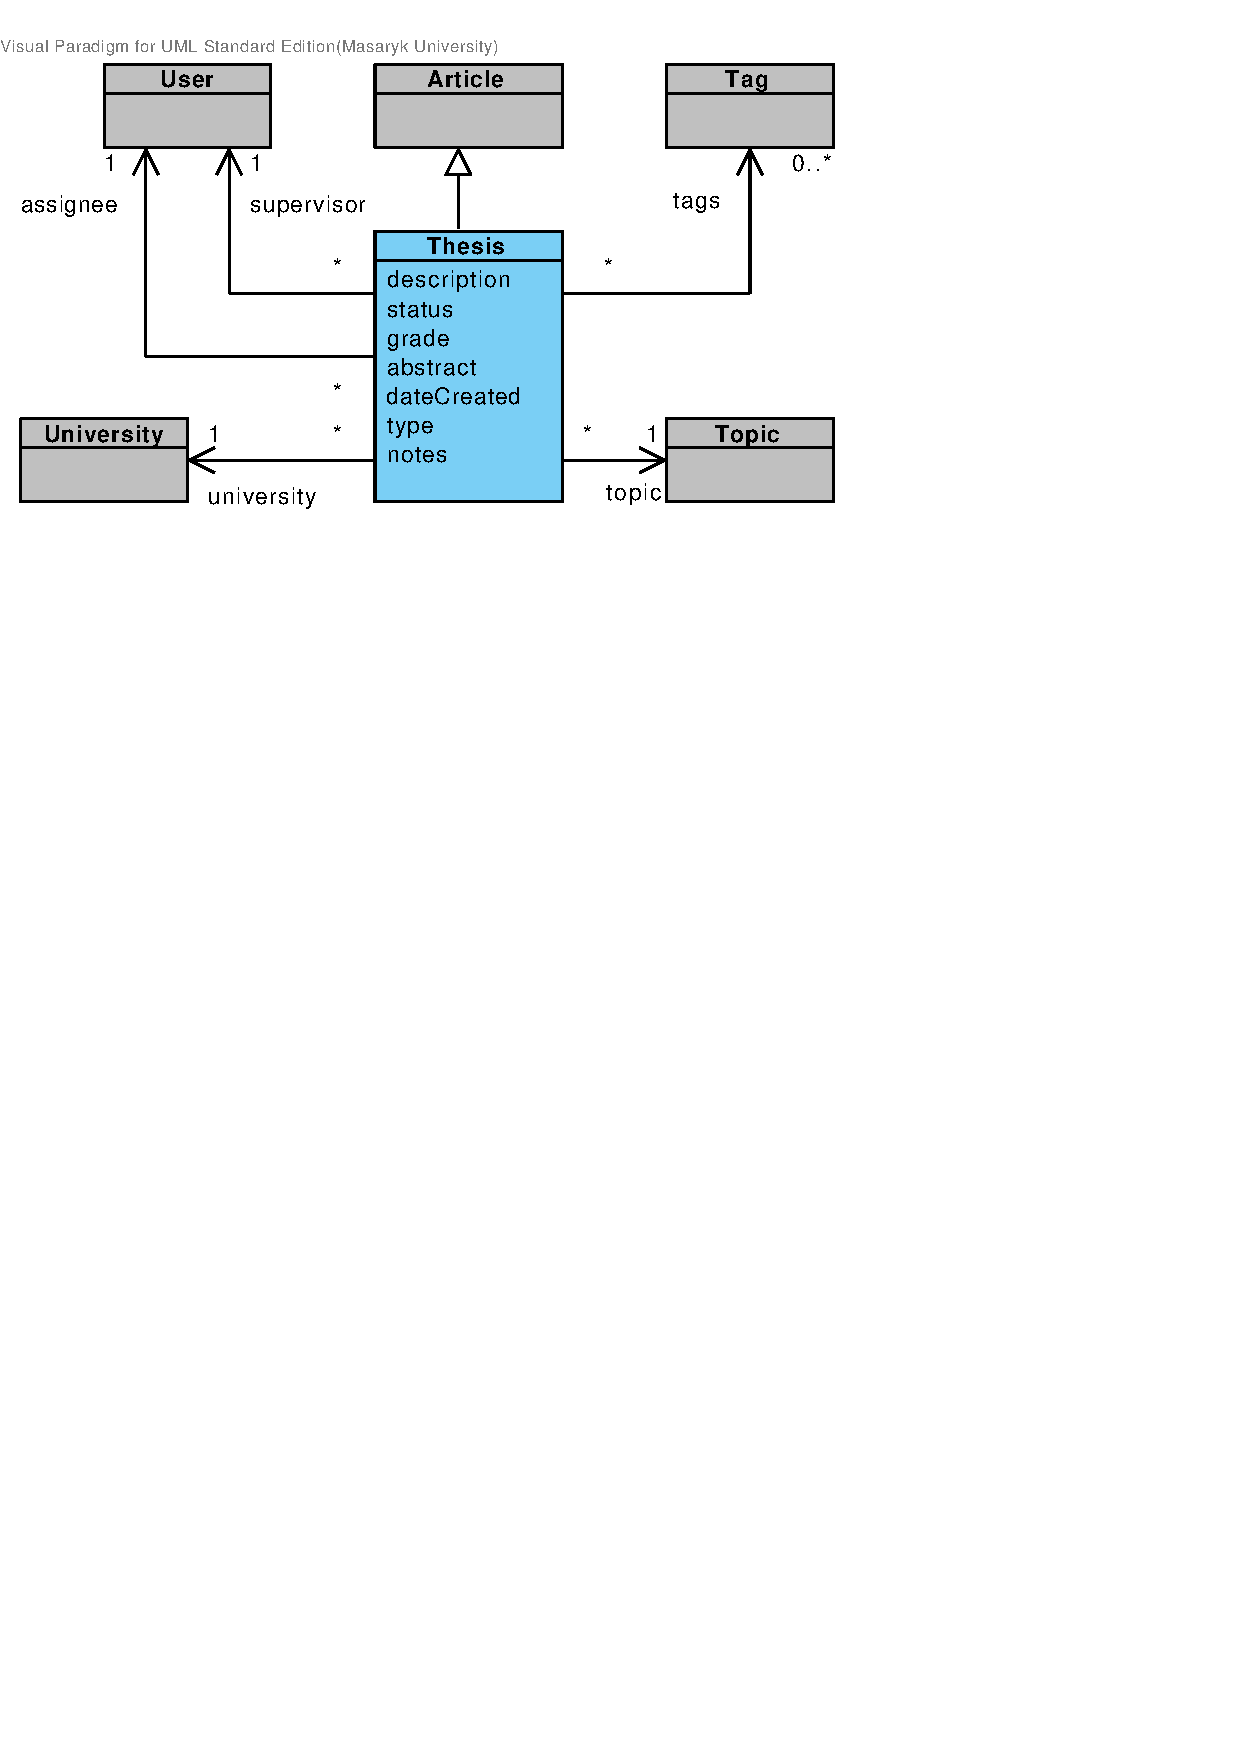
\includegraphics[trim=0 600 190 30, clip, keepaspectratio, width=\textwidth]{./images/domain-thesis-entity.pdf}
    \caption{Model of \texttt{Thesis} entity}
    \label{fig:domain-thesis-entity}
\end{figure}

\subsubsection{\textbf{\texttt{Application} entity}}

When a student applies for a topic, an application must be created to allow the leader or a supervisor to review and possibly approve it. To apply for a topic, a student must choose the type and the university for which they apply. The type is stored in the \texttt{type} field and the university is represented by the association with the \texttt{University} entity. The student can also leave a note, e.g. the preferred supervisor, which is stored in the \texttt{note} field. The \texttt{dateCreated} field allows the authority (leader or supervisor) to see what application was created first and the \texttt{approved} field marks applications that were already approved. The association with the \texttt{User} and the \texttt{Topic} entity represents the student who applied for the topic and the topic that the application is created for, respectively. The association with the \texttt{Thesis} entity allows us to display the thesis that was created from an application. Note that this association has a 0..1 multiplicity (in both directions). This is because when a student applies for a topic, the thesis has not been created yet, because it is created as soon as the leader or a supervisor approves it. The multiplicity from the other direction results from the fact that a thesis can be created directly from a topic (i.e. no application is created). This model is depicted in Figure \ref{fig:domain-application-entity}.

\begin{figure}[h]
    \centering
        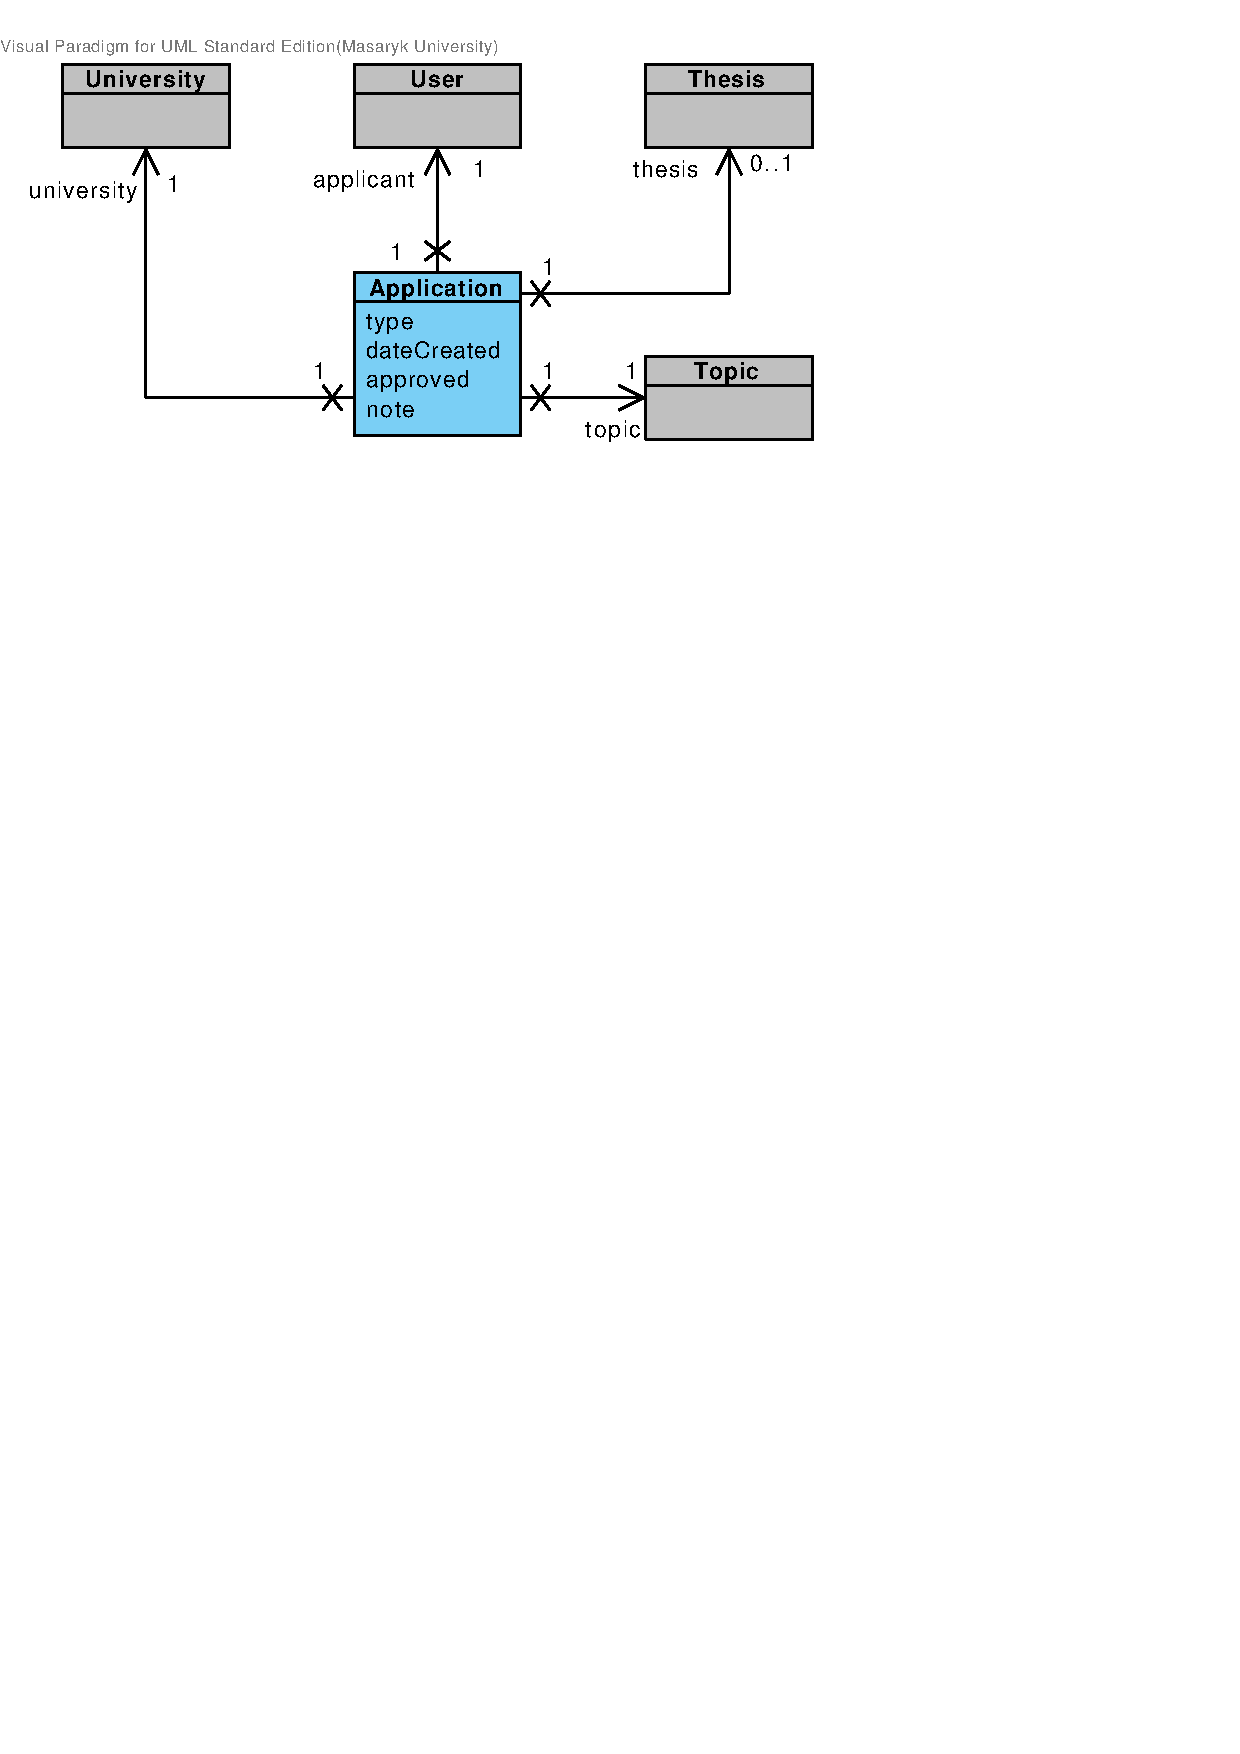
\includegraphics[trim=10 630 200 30, clip, keepaspectratio, width=\textwidth]{./images/domain-application-entity.pdf}
    \caption{Model of \texttt{Application} entity}
    \label{fig:domain-application-entity}
\end{figure}

\subsubsection{\textbf{\texttt{Faq} entity}}

To allow new users to adapt to a new system more quickly, Frequently Asked Questions are introduced. The FAQ are represented by the \texttt{Faq} entity with the following fields:

\begin{itemize}
    \item \texttt{question} -- The question to be answered.
    \item \texttt{answer} -- The answer to the frequently asked question.
    \item \texttt{locale} -- The locale of the group of users for which the frequently asked question is displayed.
\end{itemize}

See figure \ref{fig:domain-faq-entity} to see the designed model.

\begin{figure}[h]
    \centering
        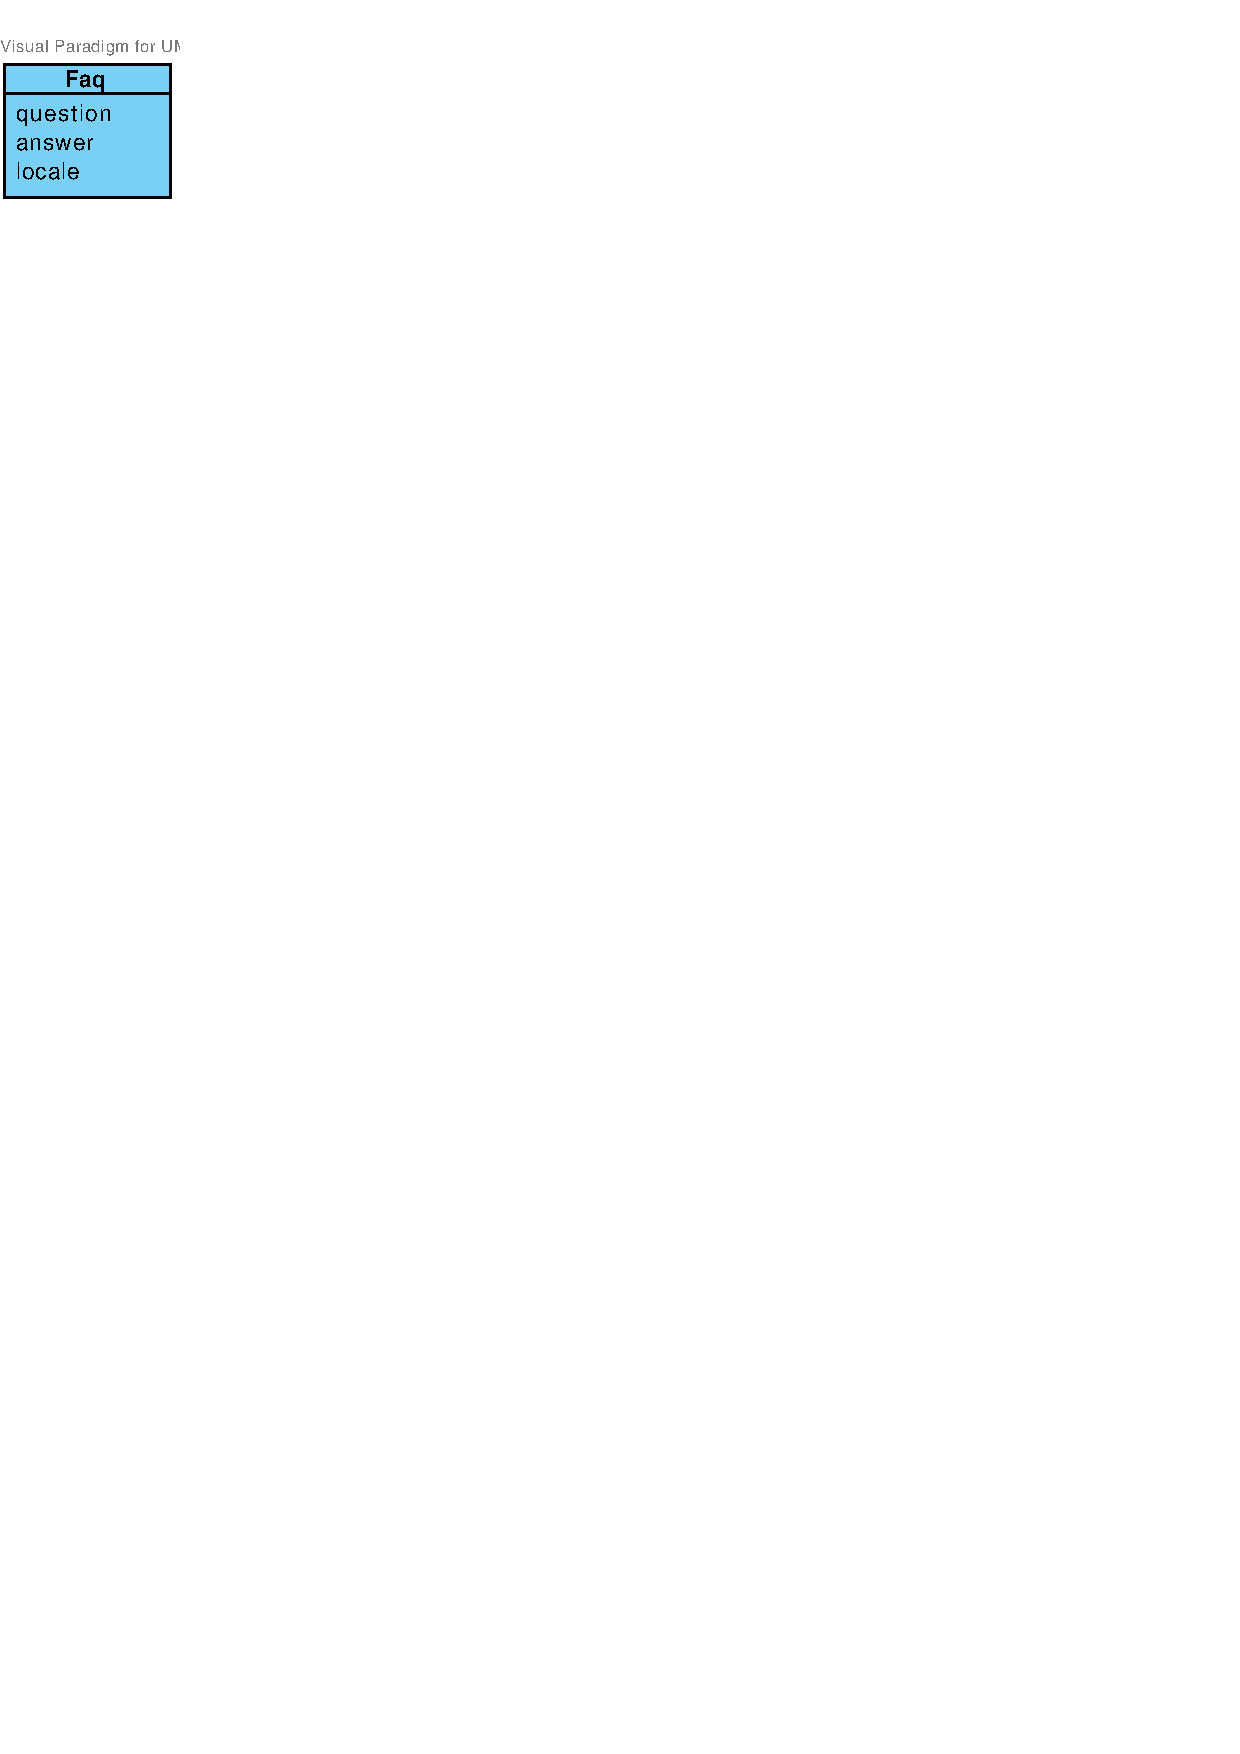
\includegraphics[trim=0 740 510 30, clip, keepaspectratio]{./images/domain-faq-entity.pdf}
    \caption{Model of \texttt{Faq} entity}
    \label{fig:domain-faq-entity}
\end{figure}

\section{Implementation}

The core project of this thesis is done by three students, therefore the implementation of it will be described in the thesis of student Jakub Cechacek.
\chapter{Future Improvements}
\label{sec:future-improvements}

Overall, the Thesis Management System is a rather large project and as it is only a bachelor thesis divided between three students, there are many features that could be implemented in the future. In this chapter, the author will investigate such possible features and describe them accordingly.

\section{Integration with Universities}

The most useful feature would be the integration of the Thesis Management System with the information systems of the universities of which Red Hat is industrial partner. This would cause all changes done in the Thesis Management System to be automatically reflected in the information systems of the universities. 

There are two ways this feature could be implemented. The first approach is to use the API of the universities, which requires to implement the integration with each university separately. This is obviously very expensive and hard to maintain, but the advantage is that there is little activity required from the universities. The second approach is to standardize and implement an API in the Thesis Management System and leave the integration to the universities. The API could follow, for example, the REST\footnote{Representational State Transfer} architecture model. The obvious disadvantage of this approach is that it could be complicated to convince the universities to do their part of implementation, which is because it could require them to do a lot of work as each university uses a different information system based on a different design model. 

If this feature were implemented, it would remove a substantial amount of logistics from the shoulders of both the universities and Red Hat, the author cannot, however, see it implemented in any other way than the later one.

\section{BPM and BRMS}

When a students works on a thesis, their supervisor usually requires them to follow a certain workflow and certain rules. This feature can be achieved by integrating the Thesis Management System with a BPM\footnote{Business Process Management} and/or a BRMS\footnote{Business Rule Management System} tool. There is a variety of BPM tools, the most considered one for our project is jBPM because it is a JBoss project and as such it is supported by Red Hat. jBPM is a light-weight, extensible workflow engine written in pure Java that allows you to execute business processes using the latest BPMN 2.0 specification\,\cite{jbpm-homepage}. For the business rule management, the Drools framework would probably be chosen as it is also supported by Red Hat\,\cite{drools-homepage}. 

It is not yet clear how the integration would be done, but as such feature would help both supervisors and students to successfully meet all requirements of their thesis, it is definitely one of the most considered one.

\section{School Projects Management}

Red Hat not only offers thesis topics to universities, but also school projects for subjects taught there. Implementation of such functionality would allow the lecturers to take advantage of the features implemented in the Thesis Management System.

To implement the project management, it would only require a new domain entity to be introduced, but how it should be integrated is not clear at the moment. It could be, as well as theses, associated with the \texttt{Topic} entity and a project would represent the concrete work of a student (or students). Another approach could be to implement project as a standalone unit, which would represent both the topic and the students' work. The former approach would present a problem with the \texttt{Topic} entity as it does not allow to persist the number of students that can apply for it. But that could be addressed by creating a child entity that would allow such functionality. The later approach, on the other hand, forces the lecturers to create new projects every semester, because a project also represents the topic and is closed at the end of each semester.

To choose the approach, elaboration with the client (Red Hat) and end users would be required. It is, however, a feature worth the effort as it would push the use case of the Thesis Management System another bit further.

\section{Import and Export of Theses and Topics}

One user of the Thesis Management System raised a feature request for the import and export of theses and theses topics in various formats. If it were the only way, apart from coping it field by field, it would allow authorized users to easily import the theses and the topics into another system.

Implementation of such a feature would be rather simple for possibly any format, because it only requires to create a template with values put in it, which is why it is placed quite near to the top of the TODO list.
\chapter{Conclusion}

The main objective of this thesis was to implement an information system for thesis management. In this document, the author briefly analyzed and described the thesis management and several software development methodologies. In the second part of the thesis, the focus was moved towards the technologies that were used for the implementation of the system, and its architecture and design in which the author covered the functional and non-functional requirements of the system and mainly its domain model. The last chapter outlined a few possibilities of improvements that could be dealt with in the future.

As with everything else, the development of the system was accompanied with several difficulties, it was, however, successfully finished and the system is currently being used by Red Hat people. Furthermore, it has proved to be reliable, scalable and usable, but only the time will tell how much those properties hold in the long run.

\bibliographystyle{IEEEtran}
\bibliography{index}

\appendix

\chapter{Diagrams}

\section{Use Case}
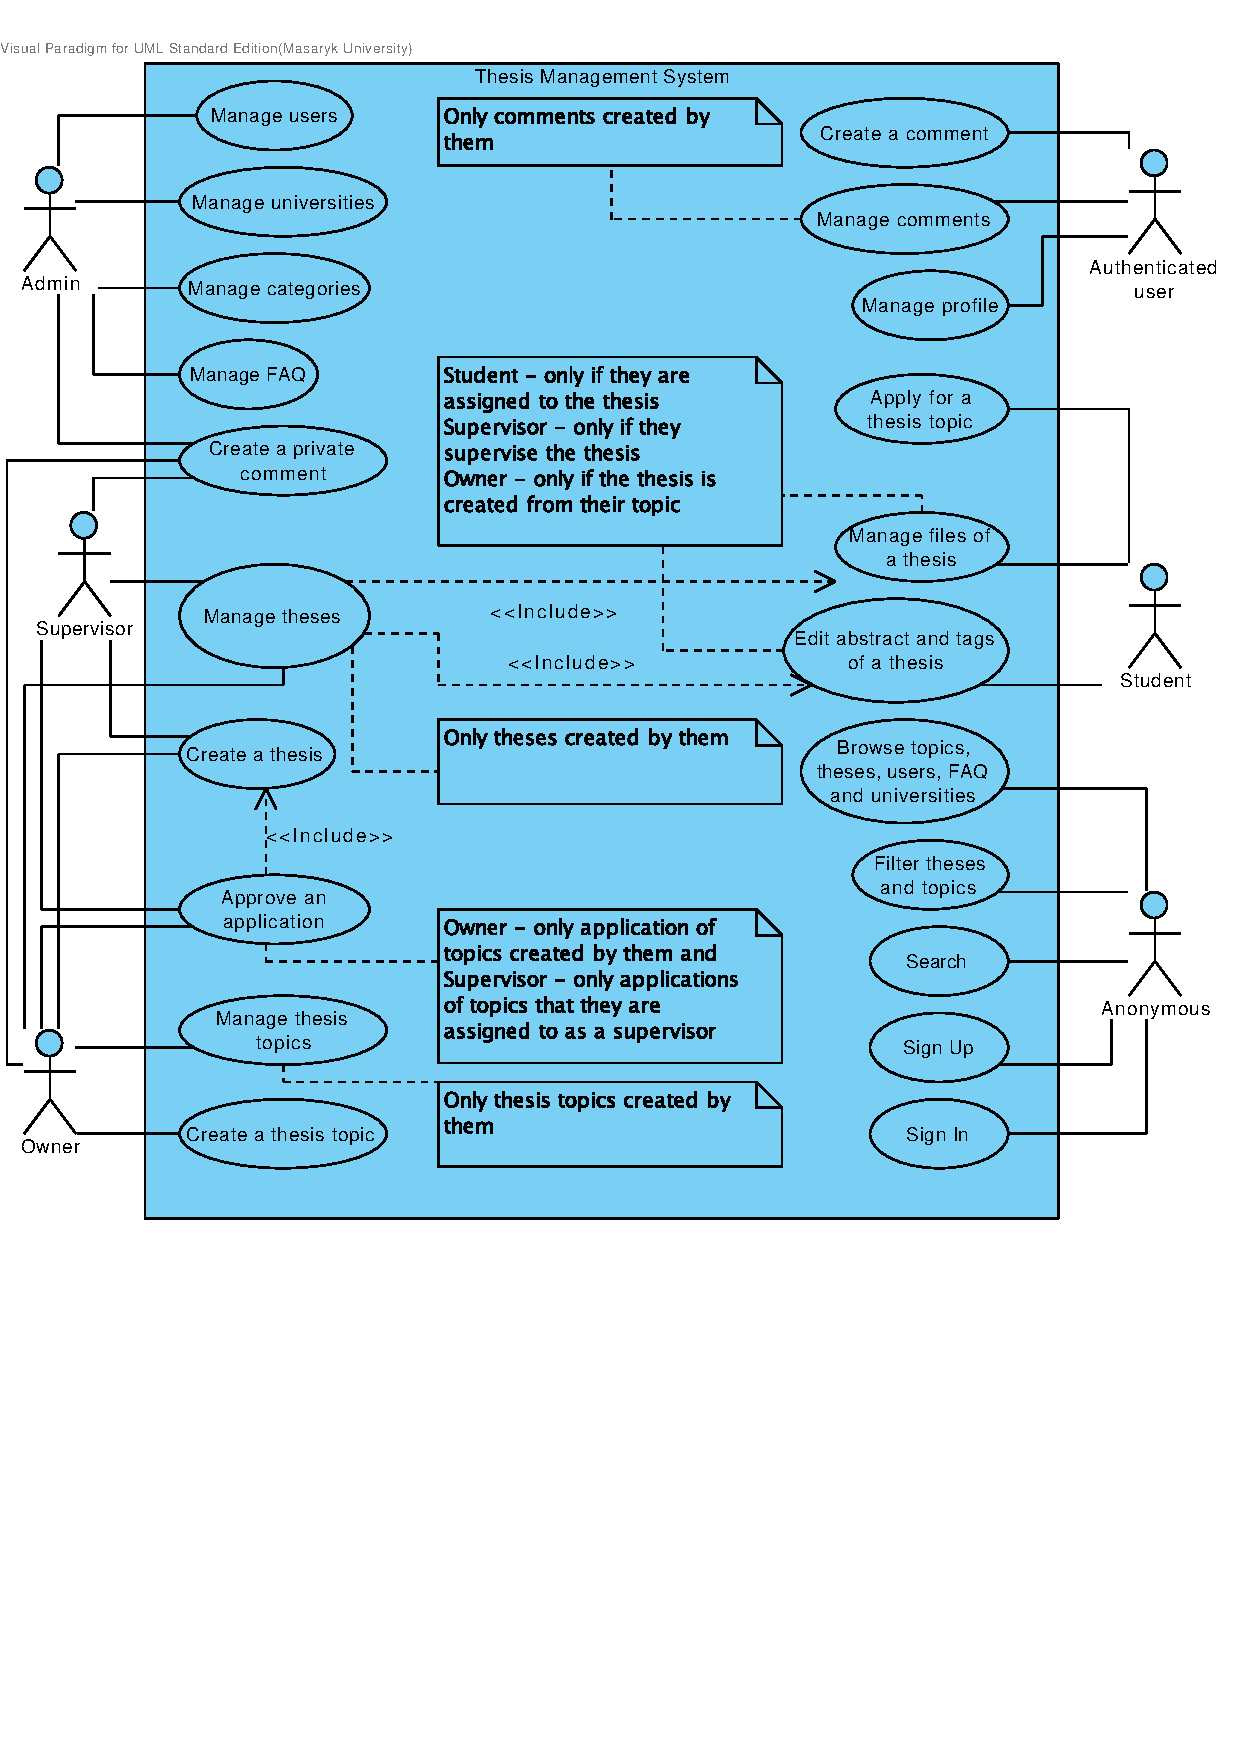
\includegraphics[keepaspectratio, trim=0 100 10 30, clip, width=\textwidth]{./images/use-case.pdf}

\section{Domain Model}
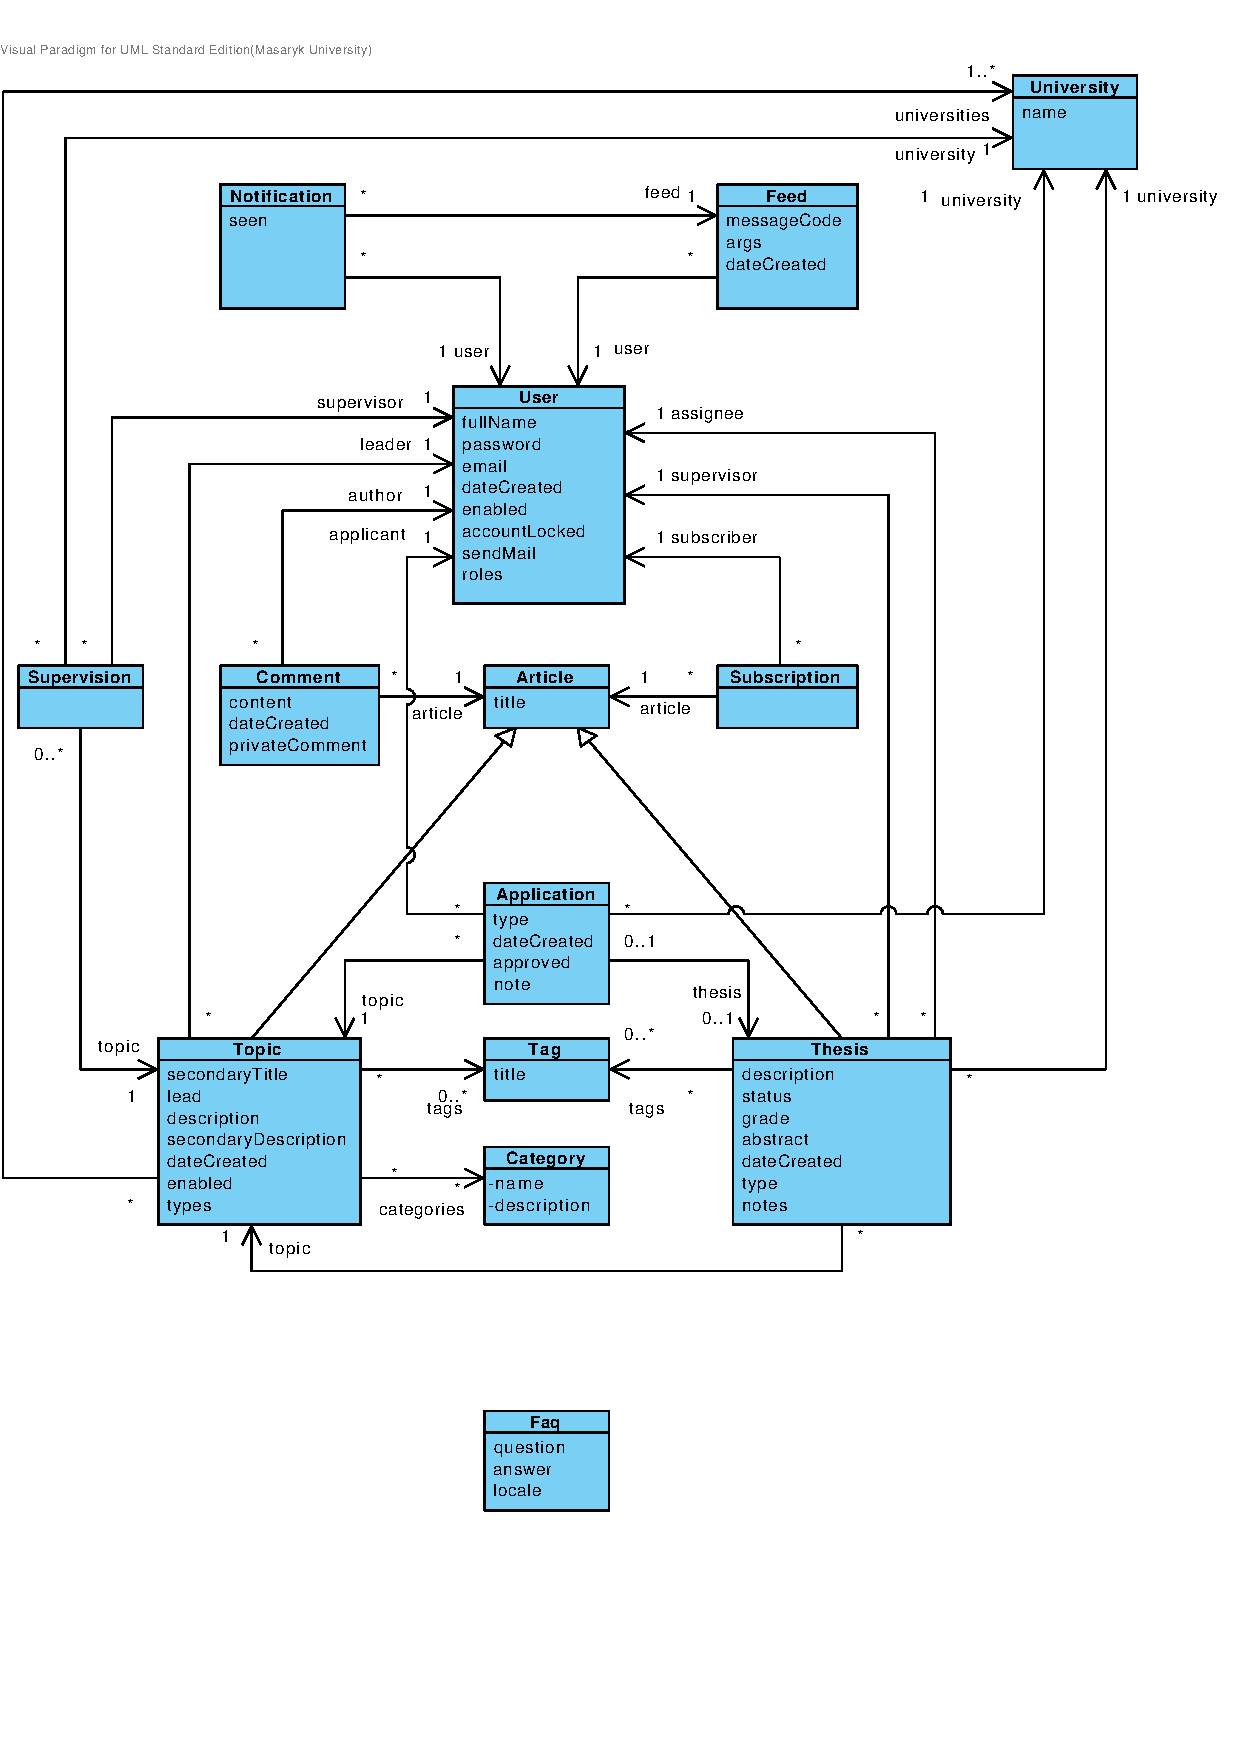
\includegraphics[keepaspectratio, trim=0 100 10 30, clip, width=\textwidth]{./images/domain-model.pdf}

\end{document}

